\section{Preventivo}
Per facilitare la lettura delle seguenti tabelle, vengono utilizzate delle sigle 
per identificare i ruoli:

\begin{table}[H]
		\begin{center}
			\setlength{\aboverulesep}{0pt}
			\setlength{\belowrulesep}{0pt}
			\setlength{\extrarowheight}{.75ex}
			\rowcolors{2}{AzzurroGruppo!10}{white}
			\begin{tabular}{ c c c }
				\rowcolor{AzzurroGruppo!30} 
				\textbf{Sigla} & \textbf{Ruolo} \\
				\toprule
				Re & Responsabile \\
				Am & Amministratore\\
				An & Analista\\
				Pt & Progettista\\
				Pr & Programmatore\\
				Ve & Verificatore\\
				\bottomrule
			\end{tabular}
			\caption{Sigle con i rispettivi ruoli}
		\end{center}
	\end{table}
\noindent
Inoltre, se le ore ricoperte in un determinato ruolo fossero nulle, la cella 
presenterà il simbolo \textbf{-} per indicarne l'assenza. 

\subsection{Fase di analisi}
\subsubsection{Prospetto orario}
In questa fase, ogni componente del gruppo rivestirà i seguenti ruoli:
\begin{table}[H]
		\begin{center}
			\setlength{\aboverulesep}{0pt}
			\setlength{\belowrulesep}{0pt}
			\setlength{\extrarowheight}{.75ex}
			\rowcolors{2}{AzzurroGruppo!10}{white}
			\begin{tabular}{ c c c c c c c c }
				\rowcolor{AzzurroGruppo!30} 
				\textbf{Nominativo} & \textbf{Re} & \textbf{Am} & \textbf{An} & \textbf{Pt} & \textbf{Pr} & \textbf{Ve} & \textbf{Ore Totali}  \\
				\toprule
				\Davide    & -  & 5  & 15 & - & - & 10 & 30 \\
				\Giosue    & -  & 8  & 17 & - & - & 5  & 30 \\
				\Francesco & 9  & 4  & 10 & - & - & 7  & 30\\
				\Daniele   & 10 & -  & 10 & - & - & 10 & 30\\
				\Lucrezia  & 10  & 3 & 7 & - & - & 10 & 30\\
				\Matteo    & -  & 5  & 12 & - & - & 13 & 30\\
				\Tommaso   & -  & 7  & 13 & - & - & 10  & 30\\
				 \textbf{Ore totali} & \textbf{29} & \textbf{32} & \textbf{84} & \textbf{-} & \textbf{-} & \textbf{65} & \textbf{210} \\
				\bottomrule
			\end{tabular}
			\caption{Distribuzione delle ore nel periodo di analisi}
		\end{center}
	\end{table}
I dati ottenuti vengono riassunti nel seguente istogramma:
\begin{figure}[H]
    \centering
    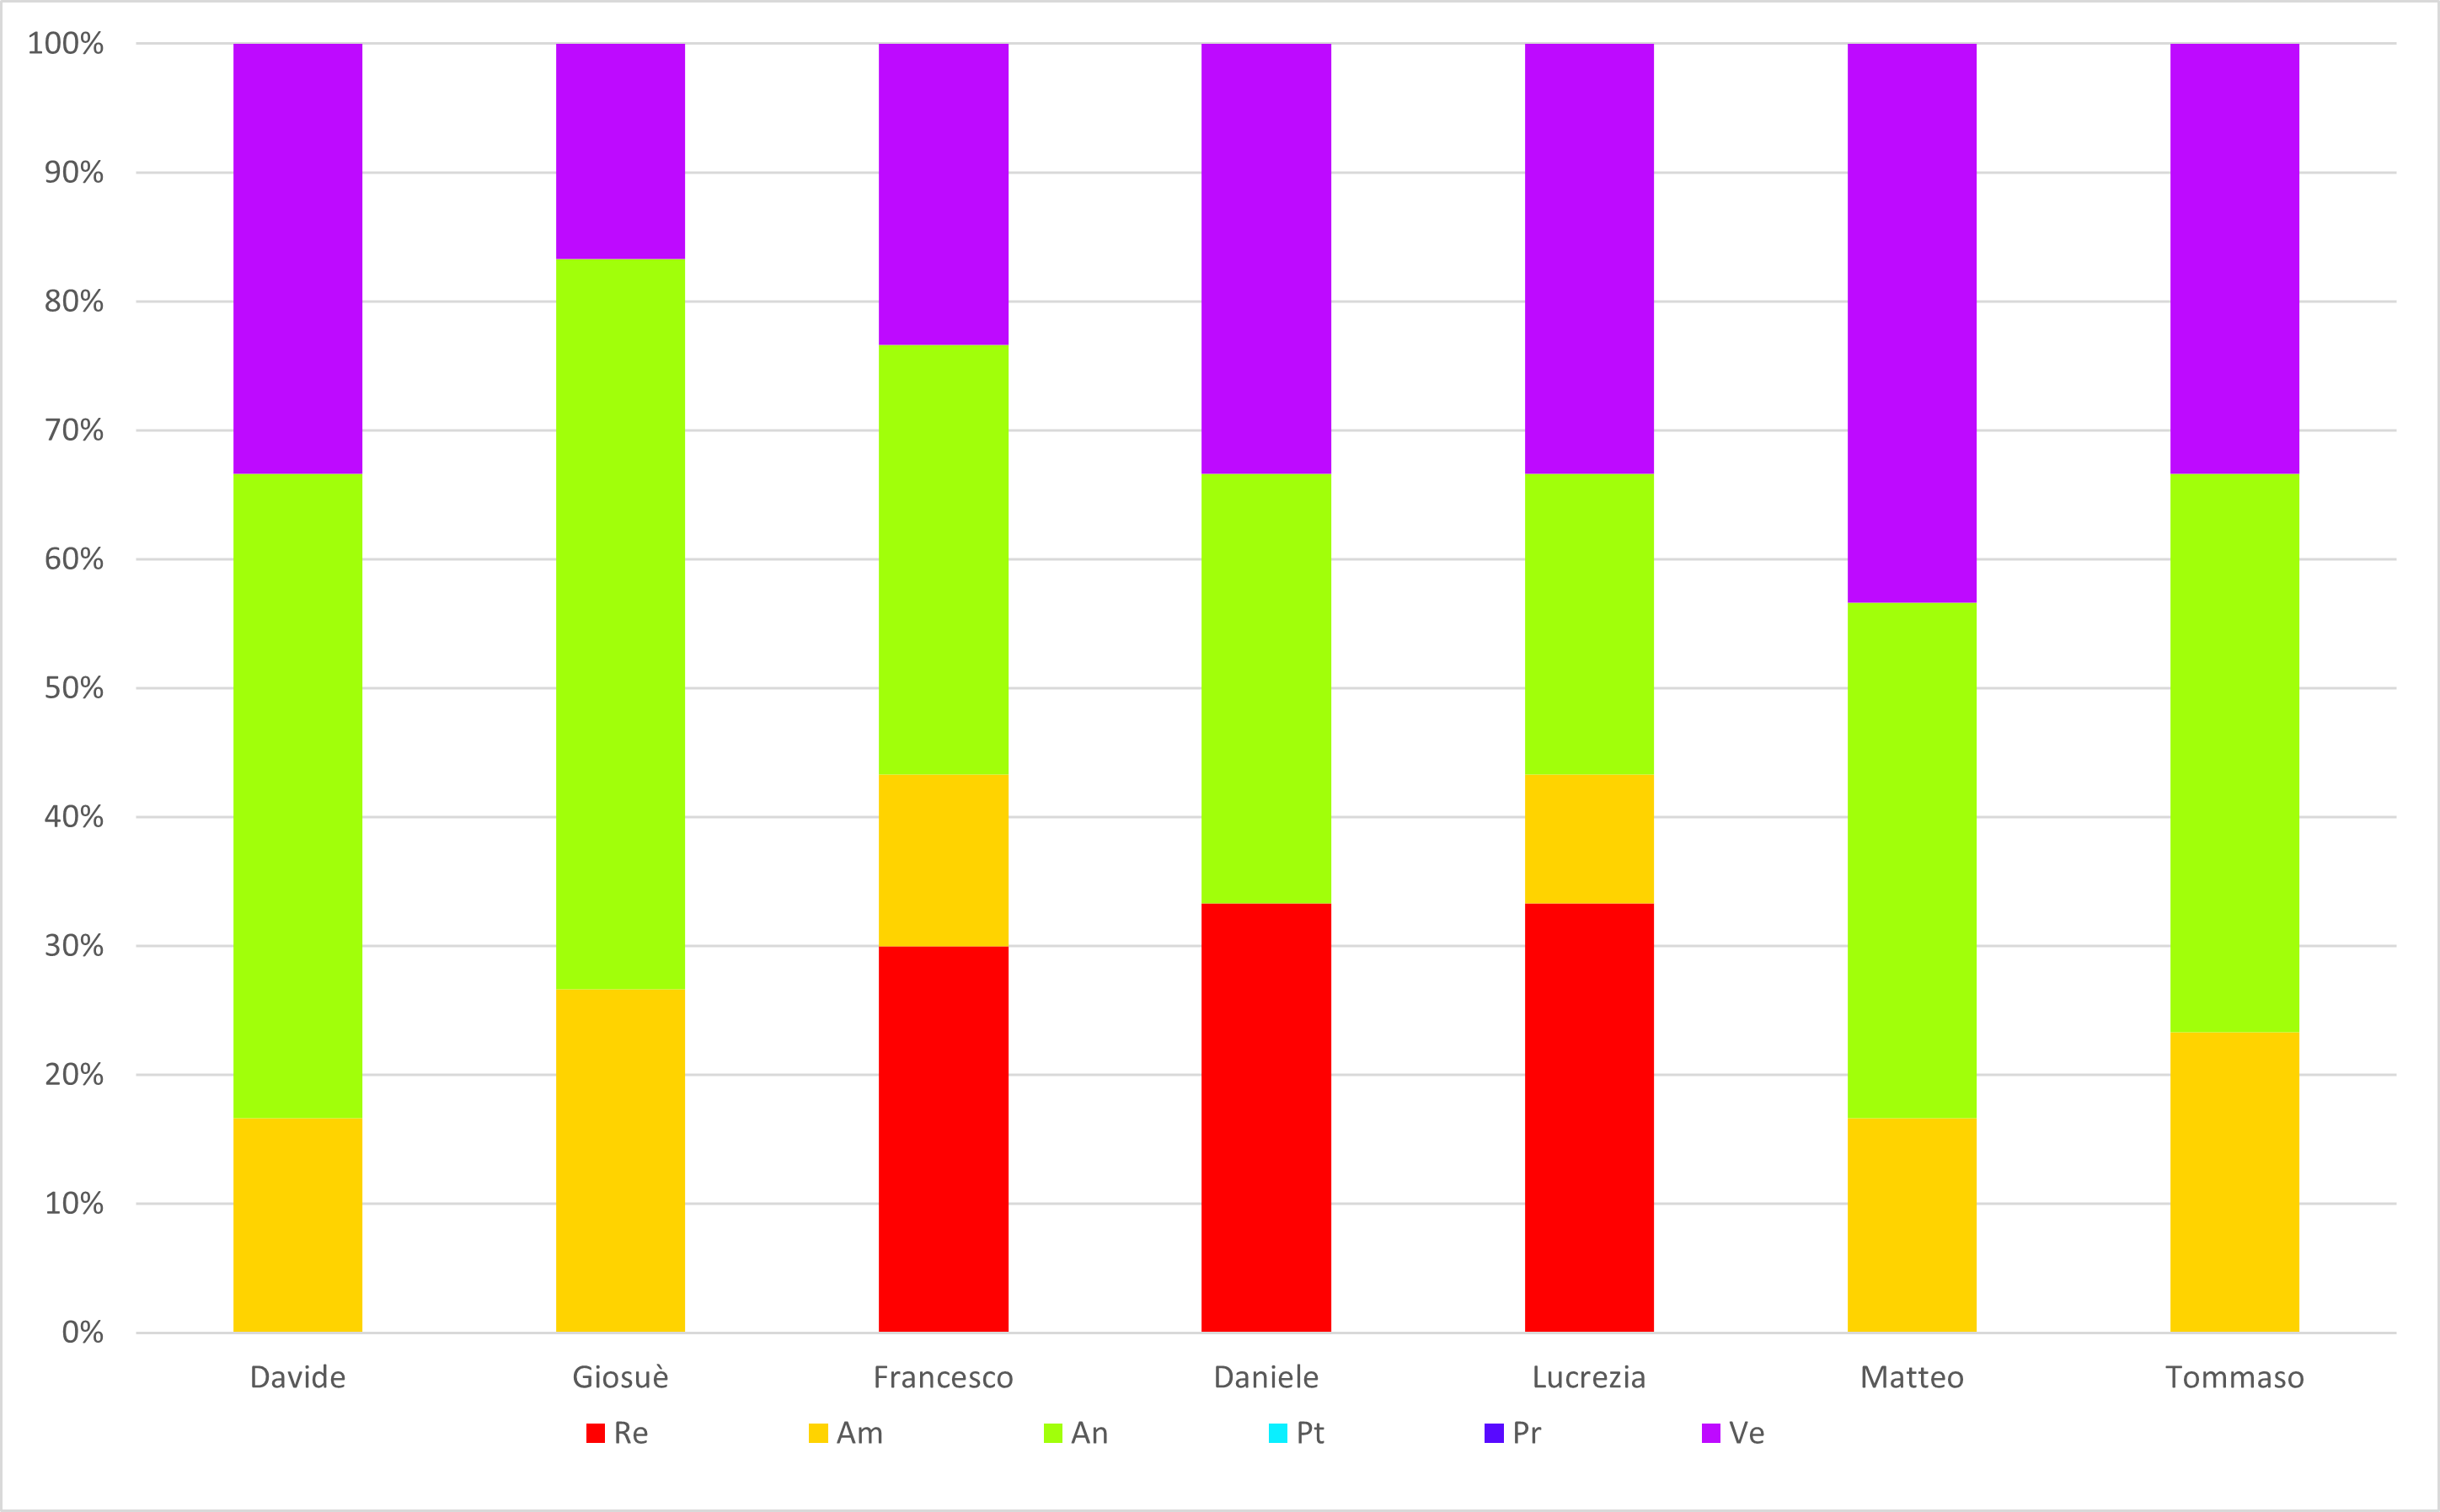
\includegraphics[scale = 0.5]{components/img/Analisi-isto.png}
    \caption{ Istogramma della ripartizione di ore per ruolo in analisi}
    \label{fig:istogramma ripartizione ore , fase di analisi}
\end{figure}
\subsubsection{Prospetto economico}
Il costo per ogni ruolo è il seguente:
\begin{table}[H]
		\begin{center}
			\setlength{\aboverulesep}{0pt}
			\setlength{\belowrulesep}{0pt}
			\setlength{\extrarowheight}{.75ex}
			\rowcolors{2}{AzzurroGruppo!10}{white}
			\begin{tabular}{ c c c }
				\rowcolor{AzzurroGruppo!30} 
				\textbf{Ruolo} & \textbf{Ore} & \textbf{Costo}  \\
				\toprule
				Responsabile & 29 & 870 \euro \\
				Amministratore & 32 & 640 \euro \\
				Analista & 84 & 2100 \euro \\
				Progettista & - & - \\
				Programmatore & - & - \\
				Verificatore & 65 & 975 \euro \\
				\textbf{Totale} & \textbf{210} & \textbf{4585 \euro} \\
				\bottomrule
			\end{tabular}
			\caption{ Prospetto dei costi per ruoli nel periodo di analisi}
		\end{center}
\end{table}
I dati ottenuti si possono riassumere nel seguente areogramma:
\begin{figure}[H]
    \centering
    \includegraphics[scale = 0.5]{components/img/analisi-torta.png}
    \caption{ Areogramma ripartizione ore, fase di analisi}
    \label{fig:Areogramma ripartizione ore, fase di analisi}
\end{figure}
\subsection{Fase di consolidamento dei requisiti}
\subsubsection{Prospetto orario}
Durante il periodo di consolidamento dei \glo{requisiti} viene effettuata la seguente distribuzione oraria:
\begin{table}[H]
		\begin{center}
			\setlength{\aboverulesep}{0pt}
			\setlength{\belowrulesep}{0pt}
			\setlength{\extrarowheight}{.75ex}
			\rowcolors{2}{AzzurroGruppo!10}{white}
			\begin{tabular}{ c c c c c c c c }
				\rowcolor{AzzurroGruppo!30} 
				\textbf{Nominativo} & \textbf{Re} & \textbf{Am} & \textbf{An} & \textbf{Pt} & \textbf{Pr} & \textbf{Ve} & \textbf{Ore Totali}  \\
				\toprule
				\Davide    & - & - & 3 & - & - & 2 & 5 \\
				\Giosue    & - & - & - & - & - & 5 & 5 \\
				\Francesco & - & - & 5 & - & - & - & 5\\
				\Daniele   & - & 3 & - & - & - & 2 & 5\\
				\Lucrezia  & 3 & - & - & - & - & 2 & 5\\
				\Matteo    & - & - & 5 & - & - & - & 5\\
				\Tommaso    & - & - & 3 & - & - & 2 & 5\\
				 \textbf{Ore totali} & \textbf{3} & \textbf{3} & \textbf{16} & \textbf{-} & \textbf{-} & \textbf{13} & \textbf{35} \\
				\bottomrule
			\end{tabular}
			\caption{Distribuzione delle ore nel periodo di consolidamento dei requisiti}
		\end{center}
	\end{table}
I dati ottenuti vengono riassunti nel seguente istogramma:
\begin{figure}[H]
    \centering
    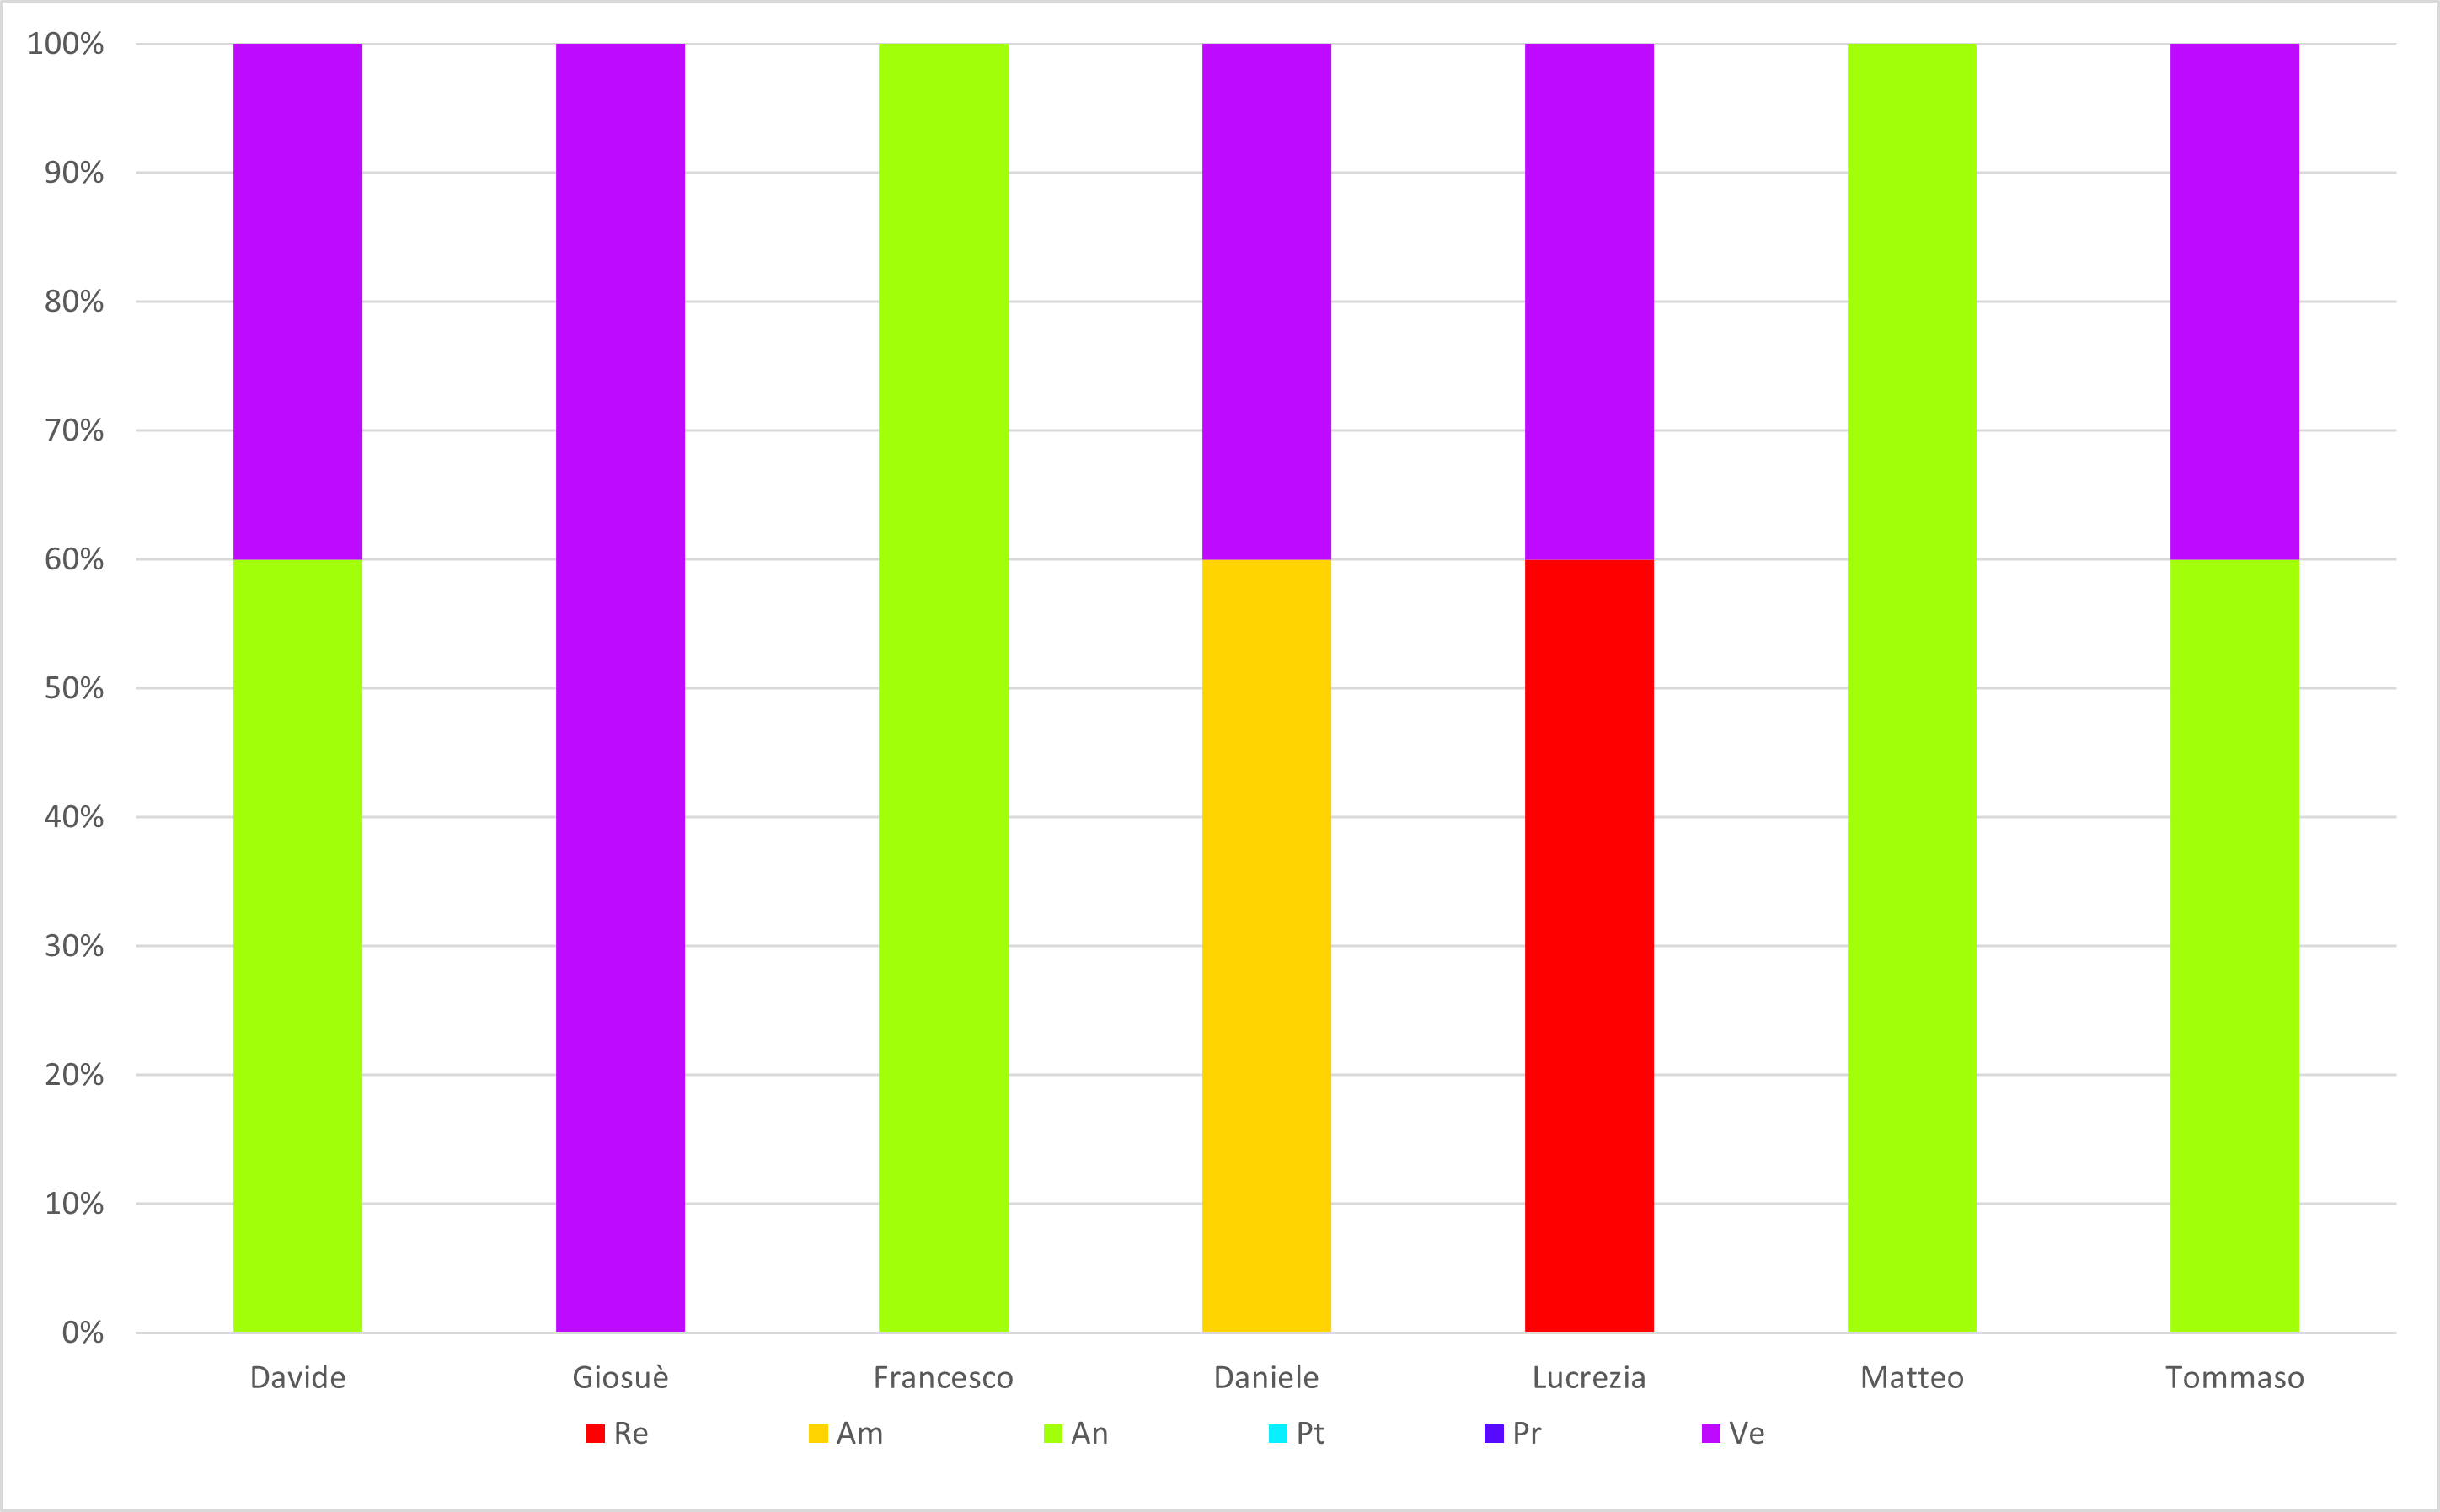
\includegraphics[scale = 0.5]{components/img/Analisi-consolidamento-isto.png}
    \caption{Istogramma della ripartizione di ore per ruolo in consolidamento dei requisiti}
    \label{fig:Istogramma ripartizione ore , fase di consolidamento dei requisiti}
\end{figure}
\subsubsection{Prospetto economico}
Il costo per ogni ruolo è il seguente:
\begin{table}[H]
		\begin{center}
			\setlength{\aboverulesep}{0pt}
			\setlength{\belowrulesep}{0pt}
			\setlength{\extrarowheight}{.75ex}
			\rowcolors{2}{AzzurroGruppo!10}{white}
			\begin{tabular}{ c c c }
				\rowcolor{AzzurroGruppo!30} 
				\textbf{Ruolo} & \textbf{Ore} & \textbf{Costo}  \\
				\toprule
				Responsabile   & 3 & 90 \euro \\
				Amministratore & 3 & 60 \euro \\
				Analista       & 16 & 400 \euro \\
				Progettista    & - & - \\
				Programmatore  & - & - \\
				Verificatore   & 13 & 195 \euro \\
				\textbf{Totale} & \textbf{35} & \textbf{745 \euro} \\
				\bottomrule
			\end{tabular}
			\caption{ Prospetto dei costi per ruoli nel periodo di consolidamento dei requisiti}
		\end{center}
	\end{table}
I dati ottenuti si possono riassumere nel seguente areogramma:
\begin{figure}[H]
    \centering
    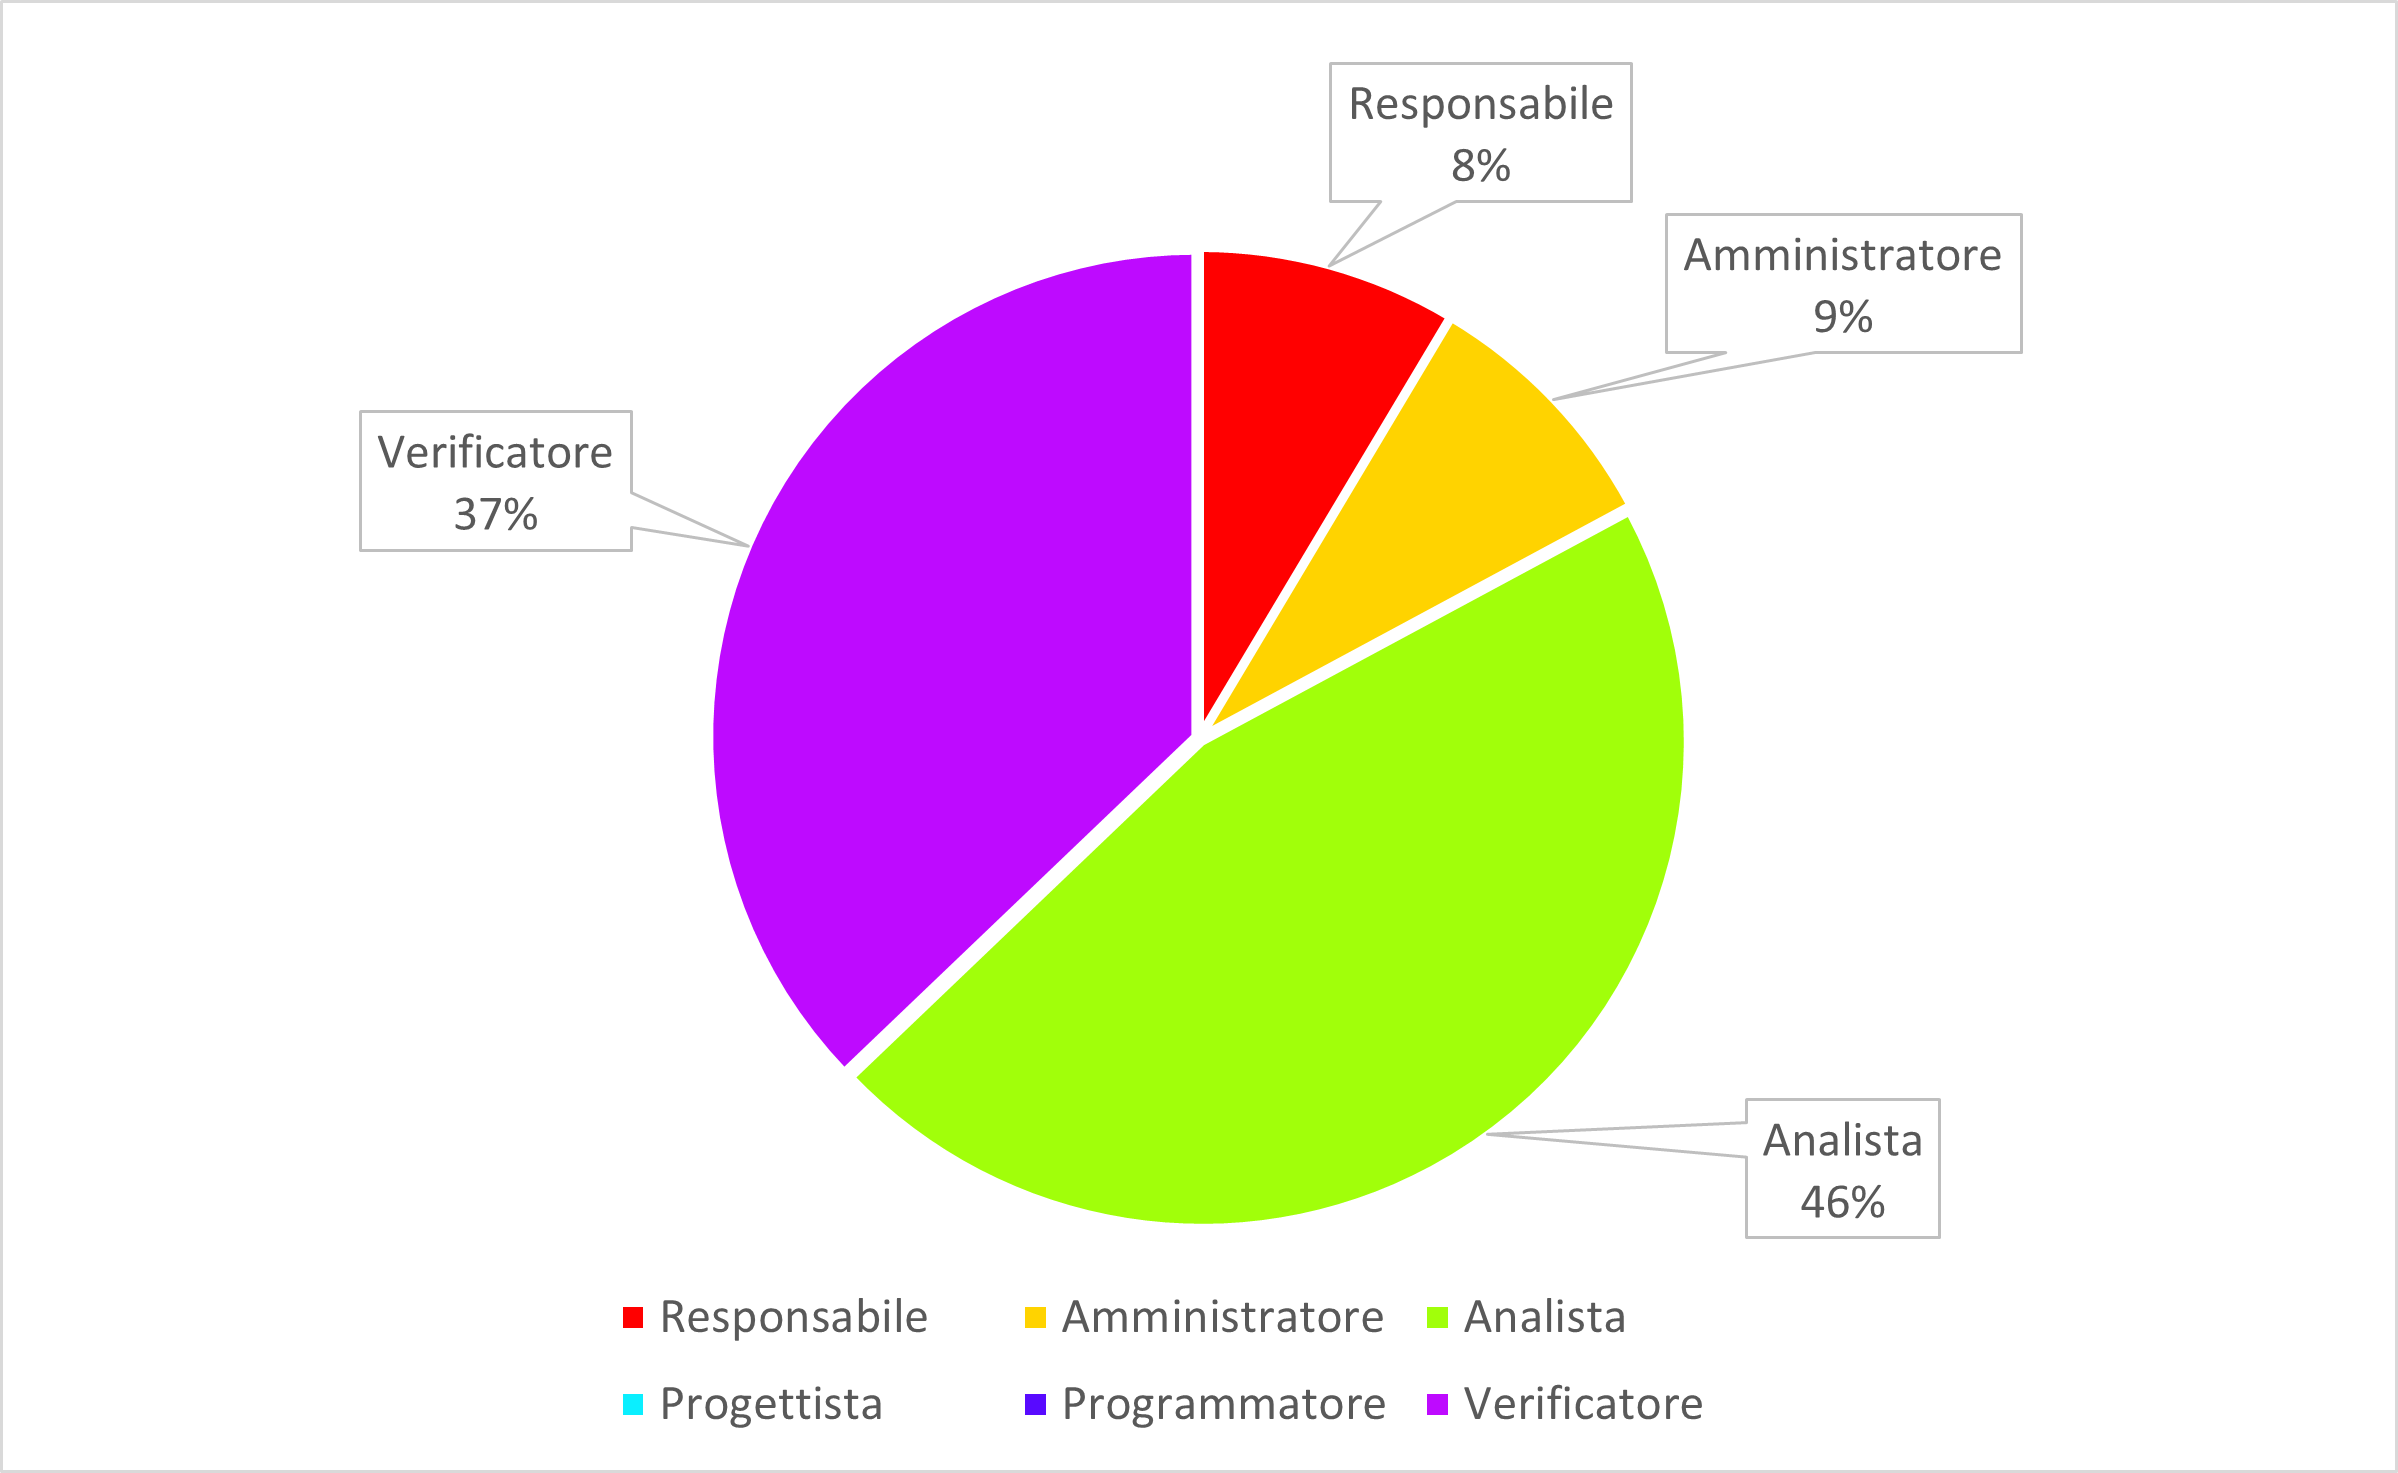
\includegraphics[scale = 0.5]{components/img/Analisi-consolidamento-torta.png}
    \caption{ Areogramma della ripartizione di ore per ruolo in consolidamento dei requisiti}
    \label{fig:Areogramma ripartizione ore, fase di consolidamento dei requisiti}
\end{figure}
\subsection{Fase di progettazione architetturale}
\subsubsection{Prospetto orario}
In questa fase la distribuzione oraria è la seguente:
\begin{table}[H]
		\begin{center}
			\setlength{\aboverulesep}{0pt}
			\setlength{\belowrulesep}{0pt}
			\setlength{\extrarowheight}{.75ex}
			\rowcolors{2}{AzzurroGruppo!10}{white}
			\begin{tabular}{ c c c c c c c c }
				\rowcolor{AzzurroGruppo!30} 
				\textbf{Nominativo} & \textbf{Re} & \textbf{Am} & \textbf{An} & \textbf{Pt} & \textbf{Pr} & \textbf{Ve} & \textbf{Ore Totali}  \\
				\toprule
				\Davide    & 5  & 6 & -  & -  & 4 & 15 & 30 \\
				\Giosue    & 3  & - & -  & 16 & 5 & 6  & 30 \\
				\Francesco & -  & - & 8  & 12 & 3 & 7  & 30\\
				\Daniele   & -  & 3 & 10 & 13 & - & 4  & 30\\
				\Lucrezia  & -  & - & 10 & -  & 4 & 16 & 30\\
				\Matteo    & 10 & 8 & -  & 12 & - & -  & 30\\
				\Tommaso   & -  & 3 & 10 & 8  & 5 & 4  & 30\\
				 \textbf{Ore totali} & \textbf{18} & \textbf{20} & \textbf{38} & \textbf{61} & \textbf{21} & \textbf{52} & \textbf{210} \\
				\bottomrule
			\end{tabular}
			\caption{Distribuzione delle ore nel periodo di  progettazione architetturale}
		\end{center}
	\end{table}
I dati ottenuti vengono riassunti nel seguente istogramma:
\begin{figure}[H]
    \centering
    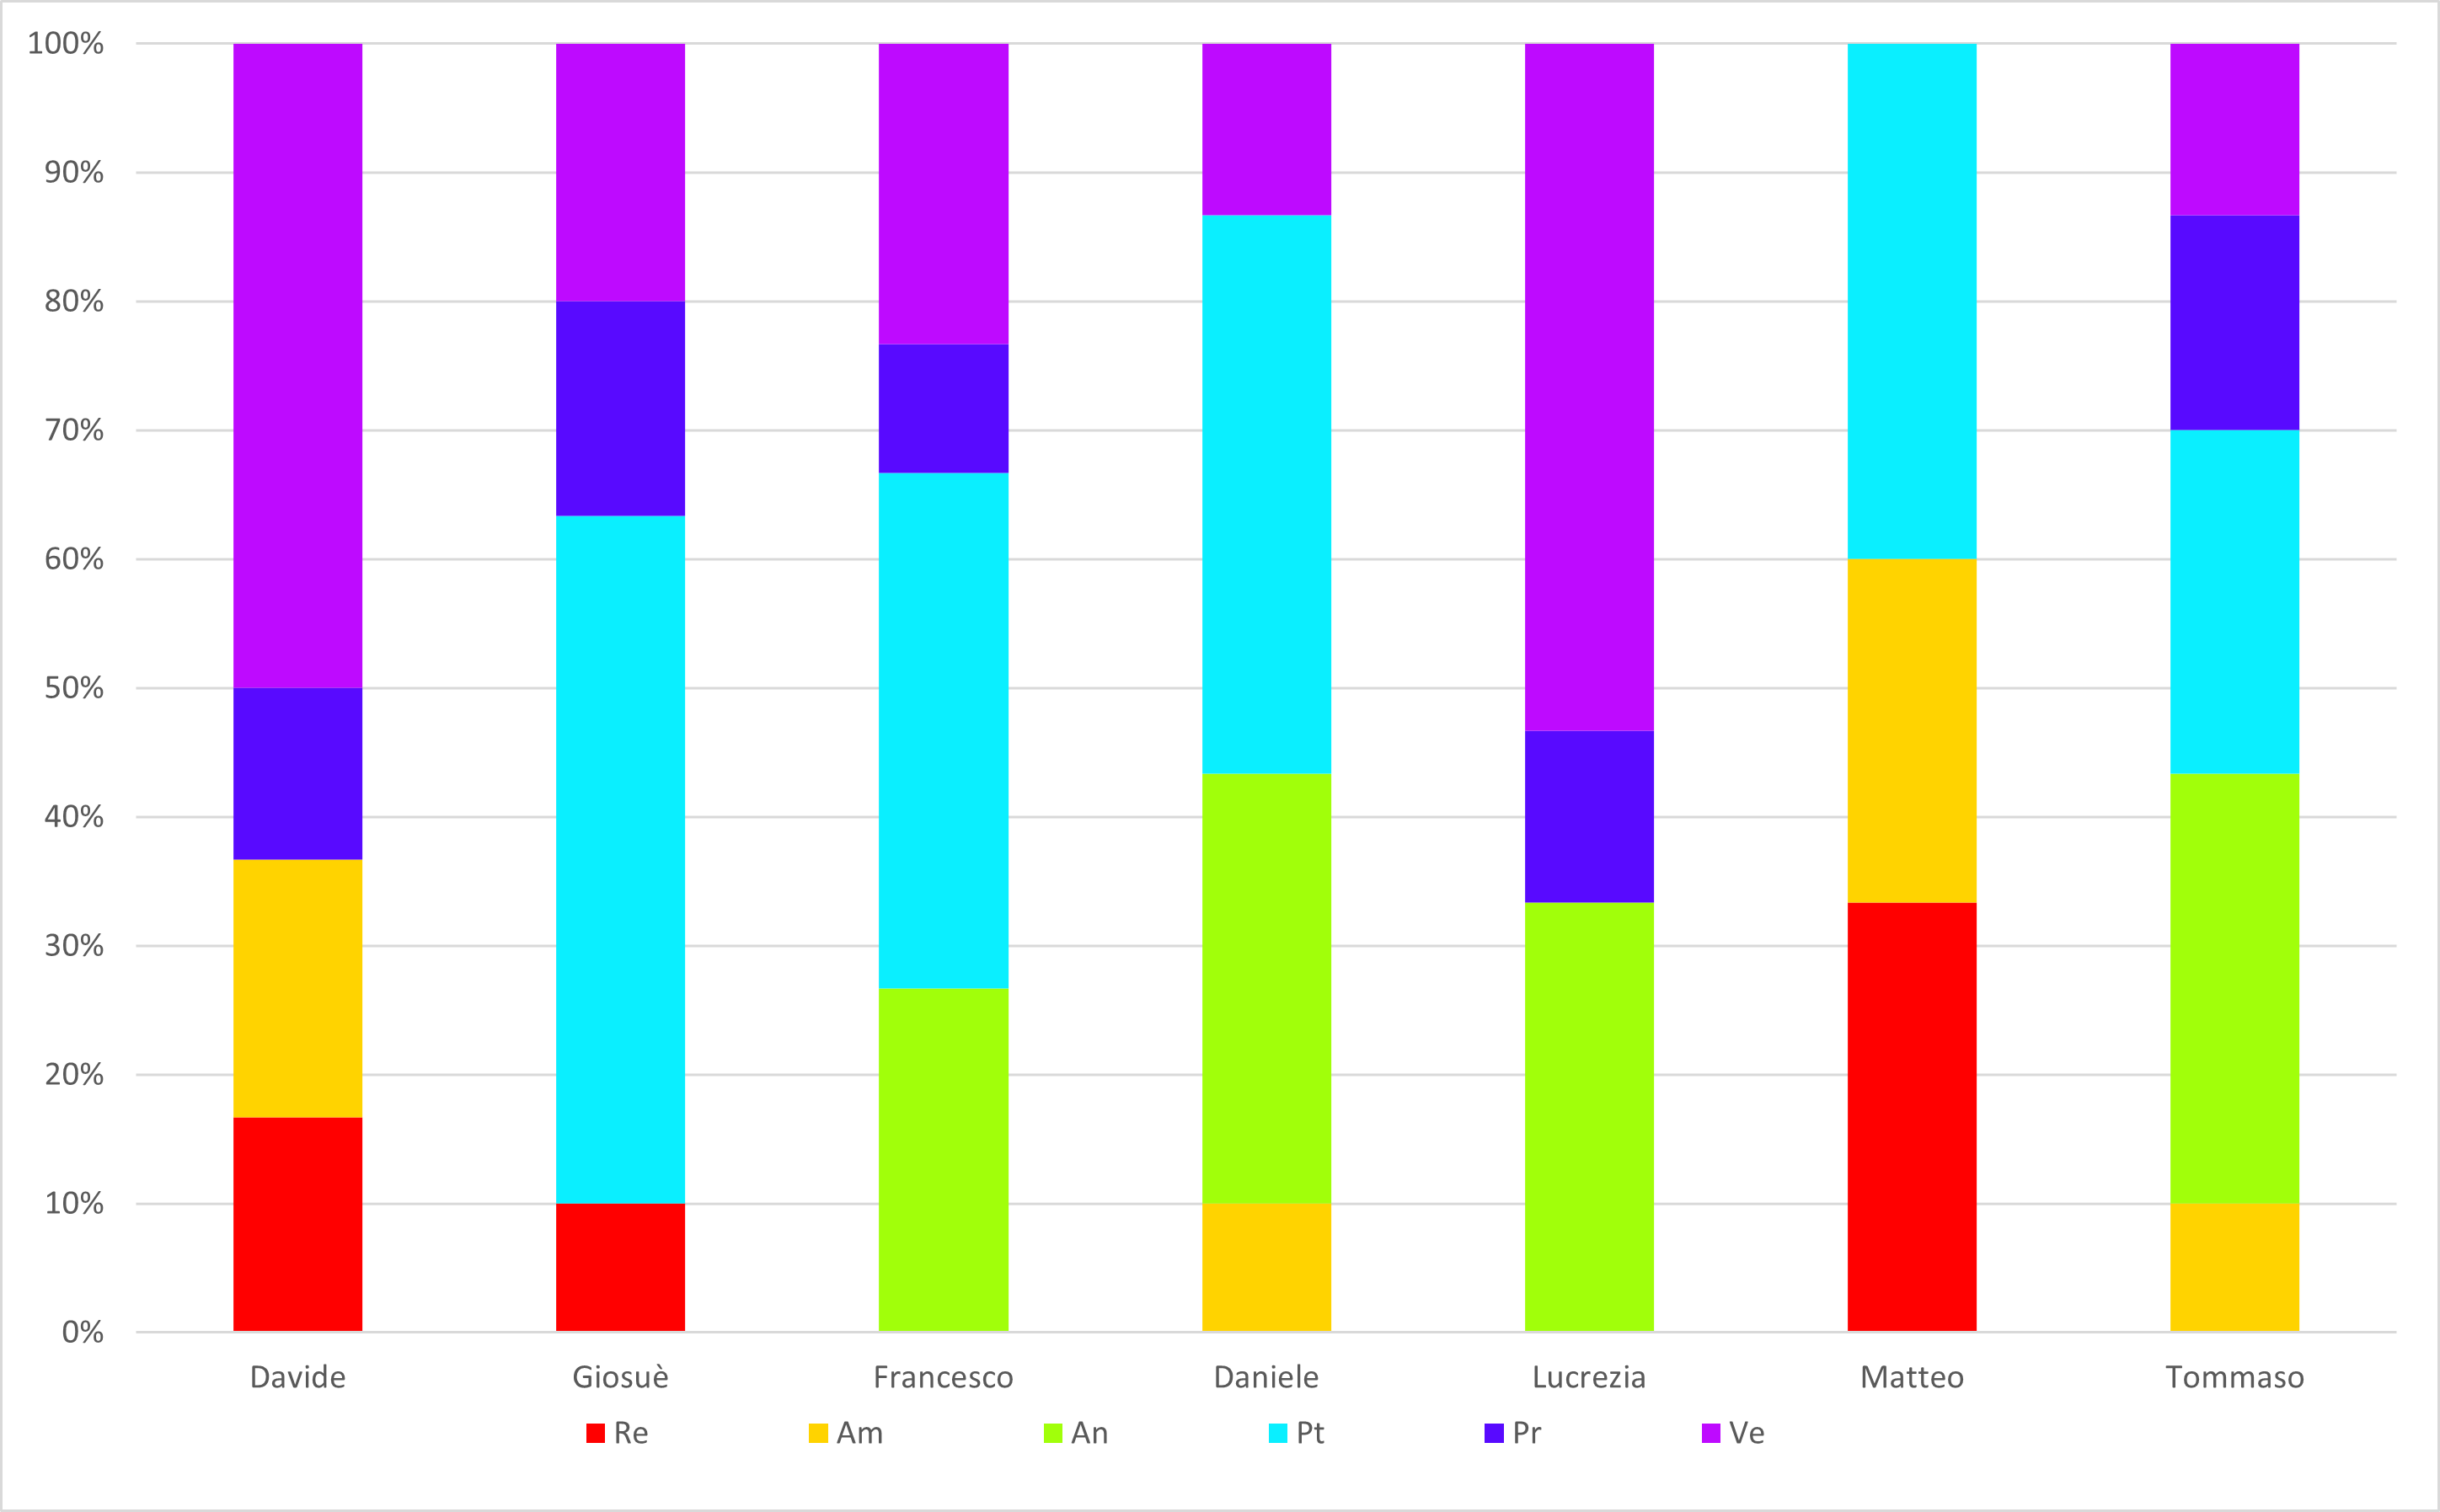
\includegraphics[scale = 0.5]{components/img/Architettura-isto.png}
    \caption{Istogramma della ripartizione di ore per ruolo in progettazione architetturale}
    \label{fig:Istogramma ripartizione ore , fase di progettazione architetturale}
\end{figure}
\subsubsection{Prospetto economico}
Il costo per ogni ruolo è il seguente:
\begin{table}[H]
		\begin{center}
			\setlength{\aboverulesep}{0pt}
			\setlength{\belowrulesep}{0pt}
			\setlength{\extrarowheight}{.75ex}
			\rowcolors{2}{AzzurroGruppo!10}{white}
			\begin{tabular}{ c c c }
				\rowcolor{AzzurroGruppo!30} 
				\textbf{Ruolo} & \textbf{Ore} & \textbf{Costo} \\
				\toprule
				Responsabile   & 18 & 540 \euro \\
				Amministratore & 20 & 400 \euro \\
				Analista       & 38 & 950 \euro \\
				Progettista    & 61 & 1342 \euro \\
				Programmatore  & 21 & 315 \euro \\
				Verificatore   & 52 & 780 \euro \\
				\textbf{Totale} & \textbf{210} & \textbf{4327 \euro} \\
				\bottomrule
			\end{tabular}
			\caption{ Prospetto dei costi per ruoli nel periodo di progettazione architetturale}
		\end{center}
	\end{table}
I dati ottenuti si possono riassumere nel seguente areogramma:
\begin{figure}[H]
    \centering
    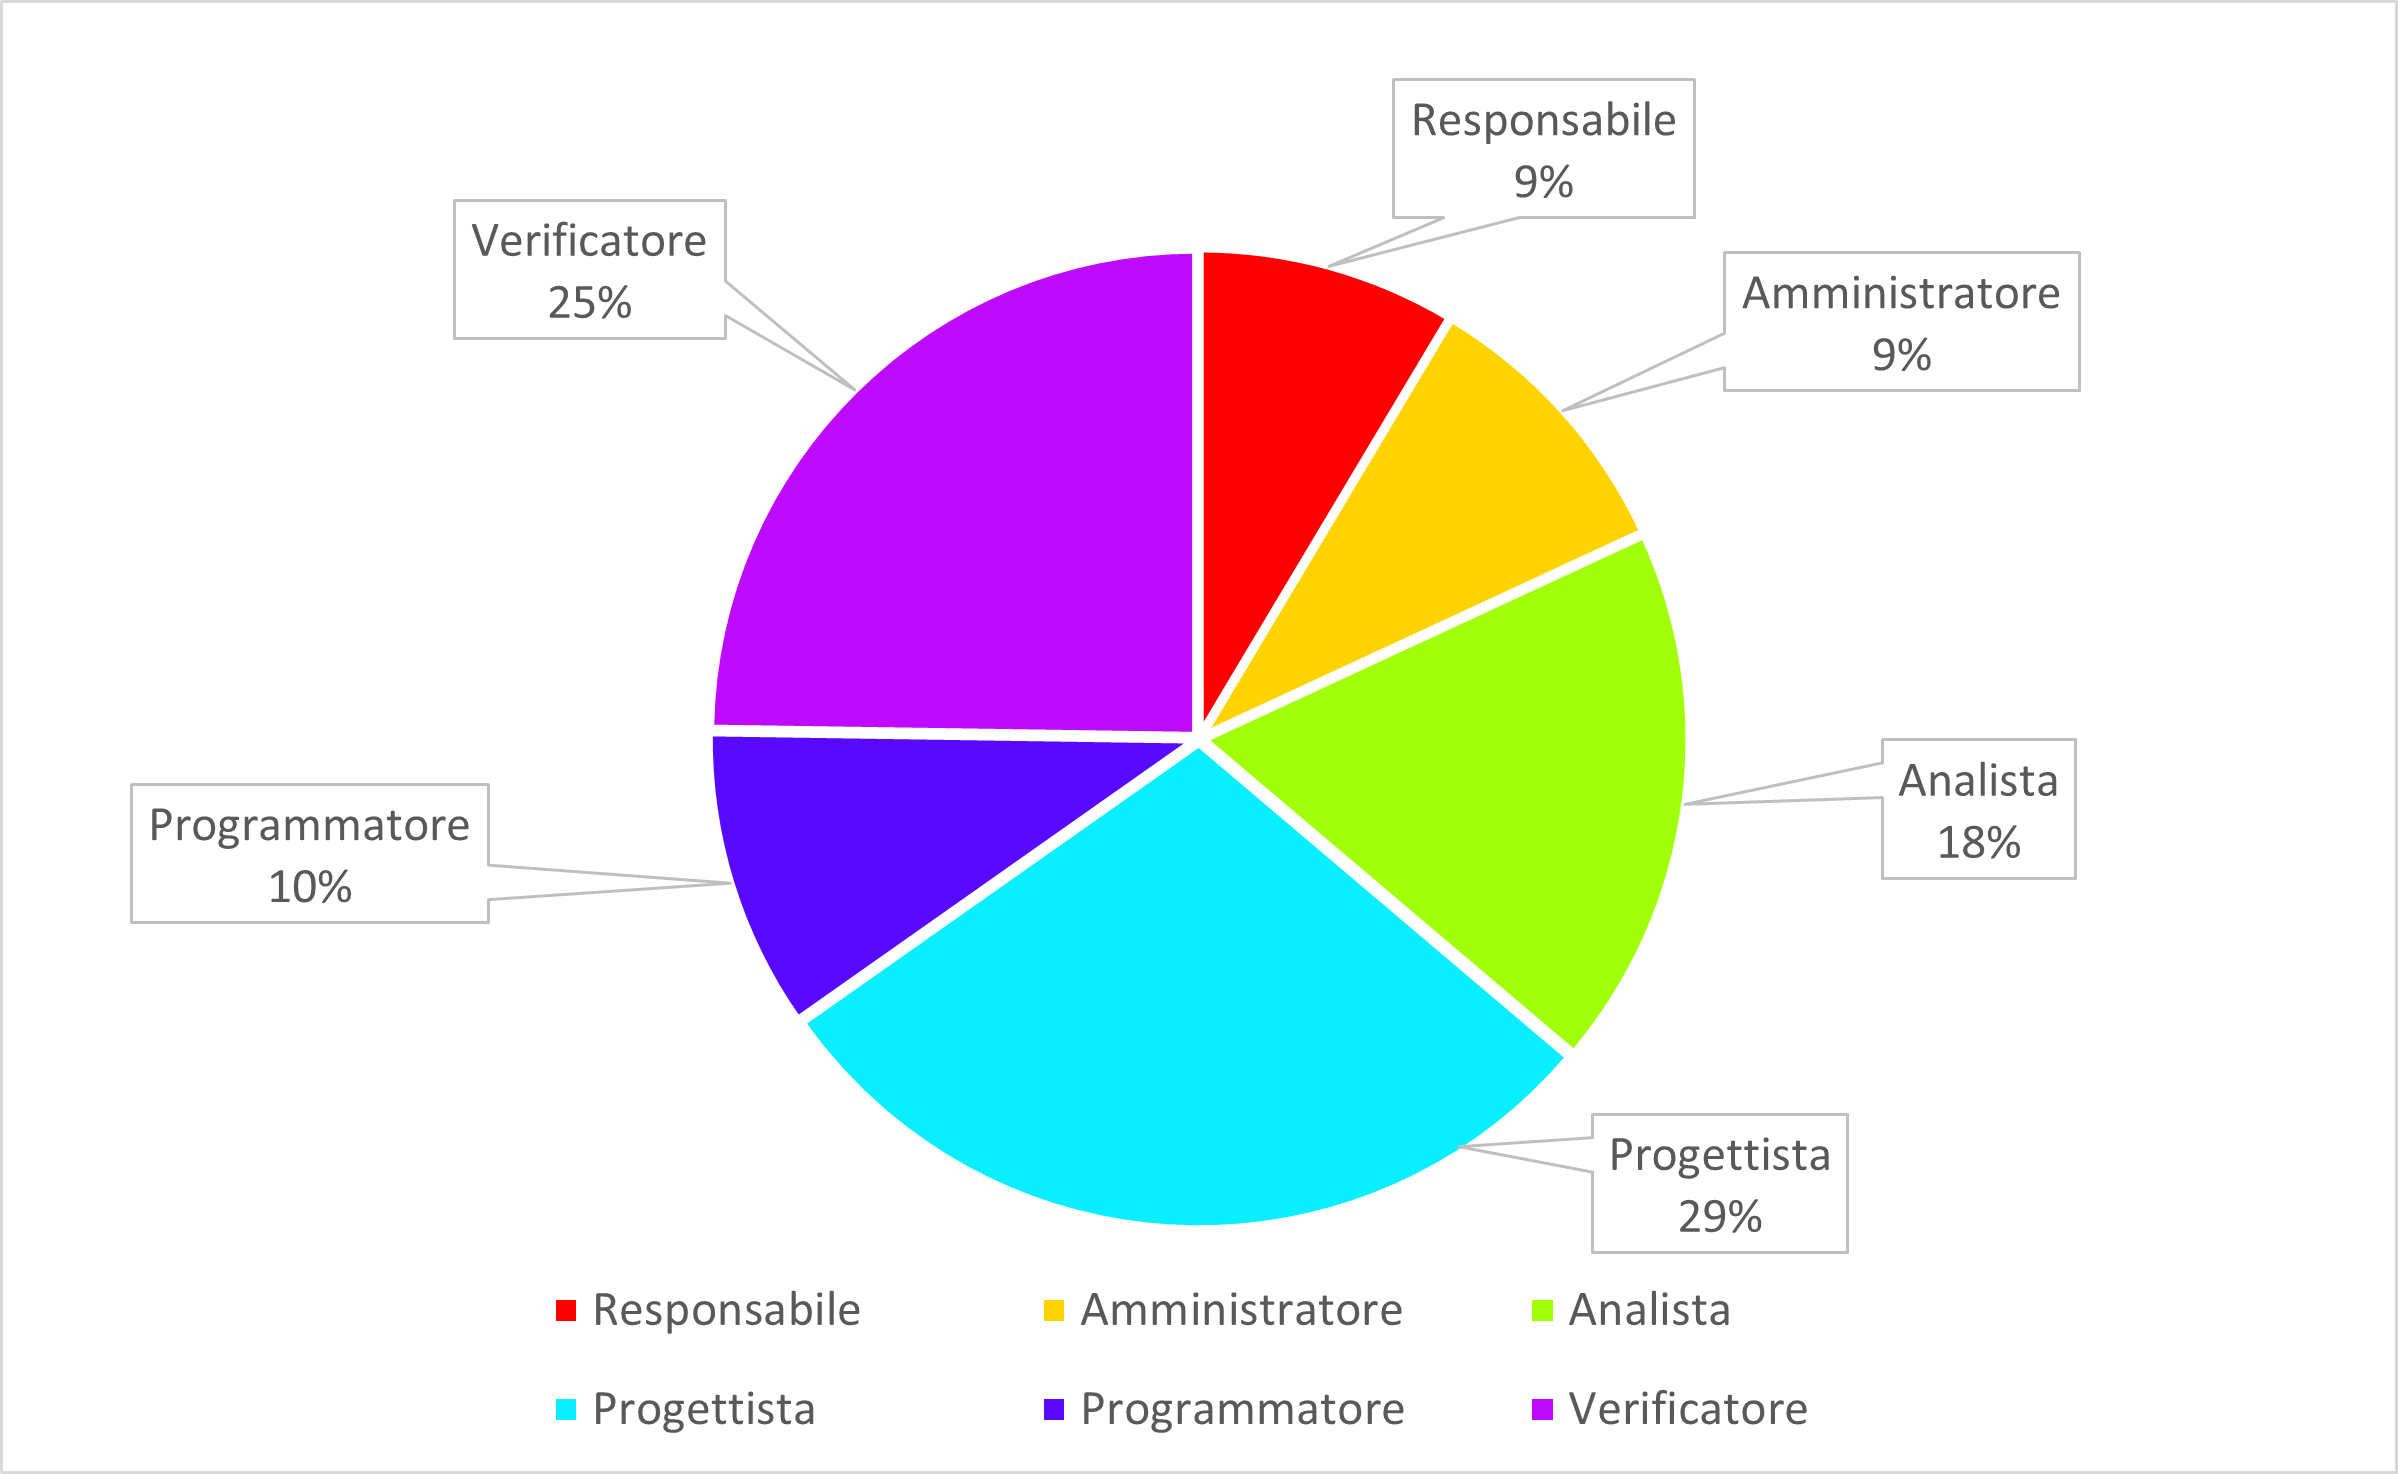
\includegraphics[scale = 0.5]{components/img/Architettura-torta.png}
    \caption{ Areogramma della ripartizione di ore per ruolo in progettazione architetturale}
    \label{fig:Areogramma ripartizione ore, fase di progettazione architetturale}
\end{figure}
\subsection{Fase di progettazione di dettaglio e codifica}

\subsubsection{Sprint 8}

In questo \glo{sprint} la distribuzione oraria è la seguente:
\begin{table}[H]
		\begin{center}
			\setlength{\aboverulesep}{0pt}
			\setlength{\belowrulesep}{0pt}
			\setlength{\extrarowheight}{.75ex}
			\rowcolors{2}{AzzurroGruppo!10}{white}
			\begin{tabular}{ c c c c c c c c }
				\rowcolor{AzzurroGruppo!30} 
				\textbf{Nominativo} & \textbf{Re} & \textbf{Am} & \textbf{An} & \textbf{Pt} & \textbf{Pr} & \textbf{Ve} & \textbf{Ore Totali}  \\
				\toprule
				\Davide    & - & - & - & 8 & 10 & 7 & 25 \\
				\Giosue    & 4 & 2 & - & 3 & 11 & 5 & 25 \\
				\Francesco & 4 & 4 & - & 6 & 6 & 5 & 25 \\
				\Daniele   & - & - & - & 7 & 10 & 8 & 25 \\
				\Lucrezia  & - & 4 & - & 7 & 8 & 6 & 25 \\
				\Matteo    & - & - & - & 7 & 13 & 5 & 25 \\
				\Tommaso   & - & - & - & 6 & 13 & 6 & 25 \\
				 \textbf{Ore totali} & \textbf{8} & \textbf{10} & \textbf{-} & \textbf{44} & \textbf{71} & \textbf{42} & \textbf{175} \\
				\bottomrule
			\end{tabular}
			\caption{Distribuzione delle ore nello sprint 8}
		\end{center}
	\end{table}


\subsubsection{Sprint 9}

In questo \glo{sprint} la distribuzione oraria è la seguente:
\begin{table}[H]
		\begin{center}
			\setlength{\aboverulesep}{0pt}
			\setlength{\belowrulesep}{0pt}
			\setlength{\extrarowheight}{.75ex}
			\rowcolors{2}{AzzurroGruppo!10}{white}
			\begin{tabular}{ c c c c c c c c }
				\rowcolor{AzzurroGruppo!30} 
				\textbf{Nominativo} & \textbf{Re} & \textbf{Am} & \textbf{An} & \textbf{Pt} & \textbf{Pr} & \textbf{Ve} & \textbf{Ore Totali}  \\
				\toprule
				\Davide    & - & - & - & 7 & 10 & 8 & 25 \\
				\Giosue    & - & - & - & 3 & 10 & 12 & 25 \\
				\Francesco & - & - & - & 6 & 14 & 5 & 25 \\
				\Daniele   & - & - & 2 & 8 & 8 & 7 & 25 \\
				\Lucrezia  & - & 4 & - & 8 & 7 & 6 & 25 \\
				\Matteo    & 4 & - & - & 8 & 8 & 5 & 25 \\
				\Tommaso   & 4 & 4 & - & 5 & 6 & 6 & 25 \\
				 \textbf{Ore totali} & \textbf{8} & \textbf{8} & \textbf{2} & \textbf{45} & \textbf{63} & \textbf{49} & \textbf{175} \\
				\bottomrule
			\end{tabular}
			\caption{Distribuzione delle ore nello sprint 9}
		\end{center}
	\end{table}


\subsubsection{Prospetto orario}
In questa fase la distribuzione oraria è la seguente:
\begin{table}[H]
		\begin{center}
			\setlength{\aboverulesep}{0pt}
			\setlength{\belowrulesep}{0pt}
			\setlength{\extrarowheight}{.75ex}
			\rowcolors{2}{AzzurroGruppo!10}{white}
			\begin{tabular}{ c c c c c c c c }
				\rowcolor{AzzurroGruppo!30} 
				\textbf{Nominativo} & \textbf{Re} & \textbf{Am} & \textbf{An} & \textbf{Pt} & \textbf{Pr} & \textbf{Ve} & \textbf{Ore Totali}  \\
				\toprule
				\Davide    & - & - & - & 15 & 20 & 15 & 50 \\
				\Giosue    & 4 & 2 & - & 6 & 21 & 17 & 50 \\
				\Francesco & 4 & 4 & - & 12 & 20 & 10 & 50 \\
				\Daniele   & - & - & 2 & 15 & 18 & 15 & 50 \\
				\Lucrezia  & - & 8 & - & 15 & 15 & 12 & 50 \\
				\Matteo    & 4 & - & - & 15 & 21 & 10 & 50 \\
				\Tommaso   & 4 & 4 & - & 11 & 19 & 12 & 50 \\
				 \textbf{Ore totali} & \textbf{16} & \textbf{18} & \textbf{2} & \textbf{89} & \textbf{134} & \textbf{91} & \textbf{350} \\
				\bottomrule
			\end{tabular}
			\caption{Distribuzione delle ore nel periodo di progettazione di dettaglio e codifica}
		\end{center}
	\end{table}
	I dati ottenuti vengono riassunti nel seguente istogramma:
\begin{figure}[H]
    \centering
    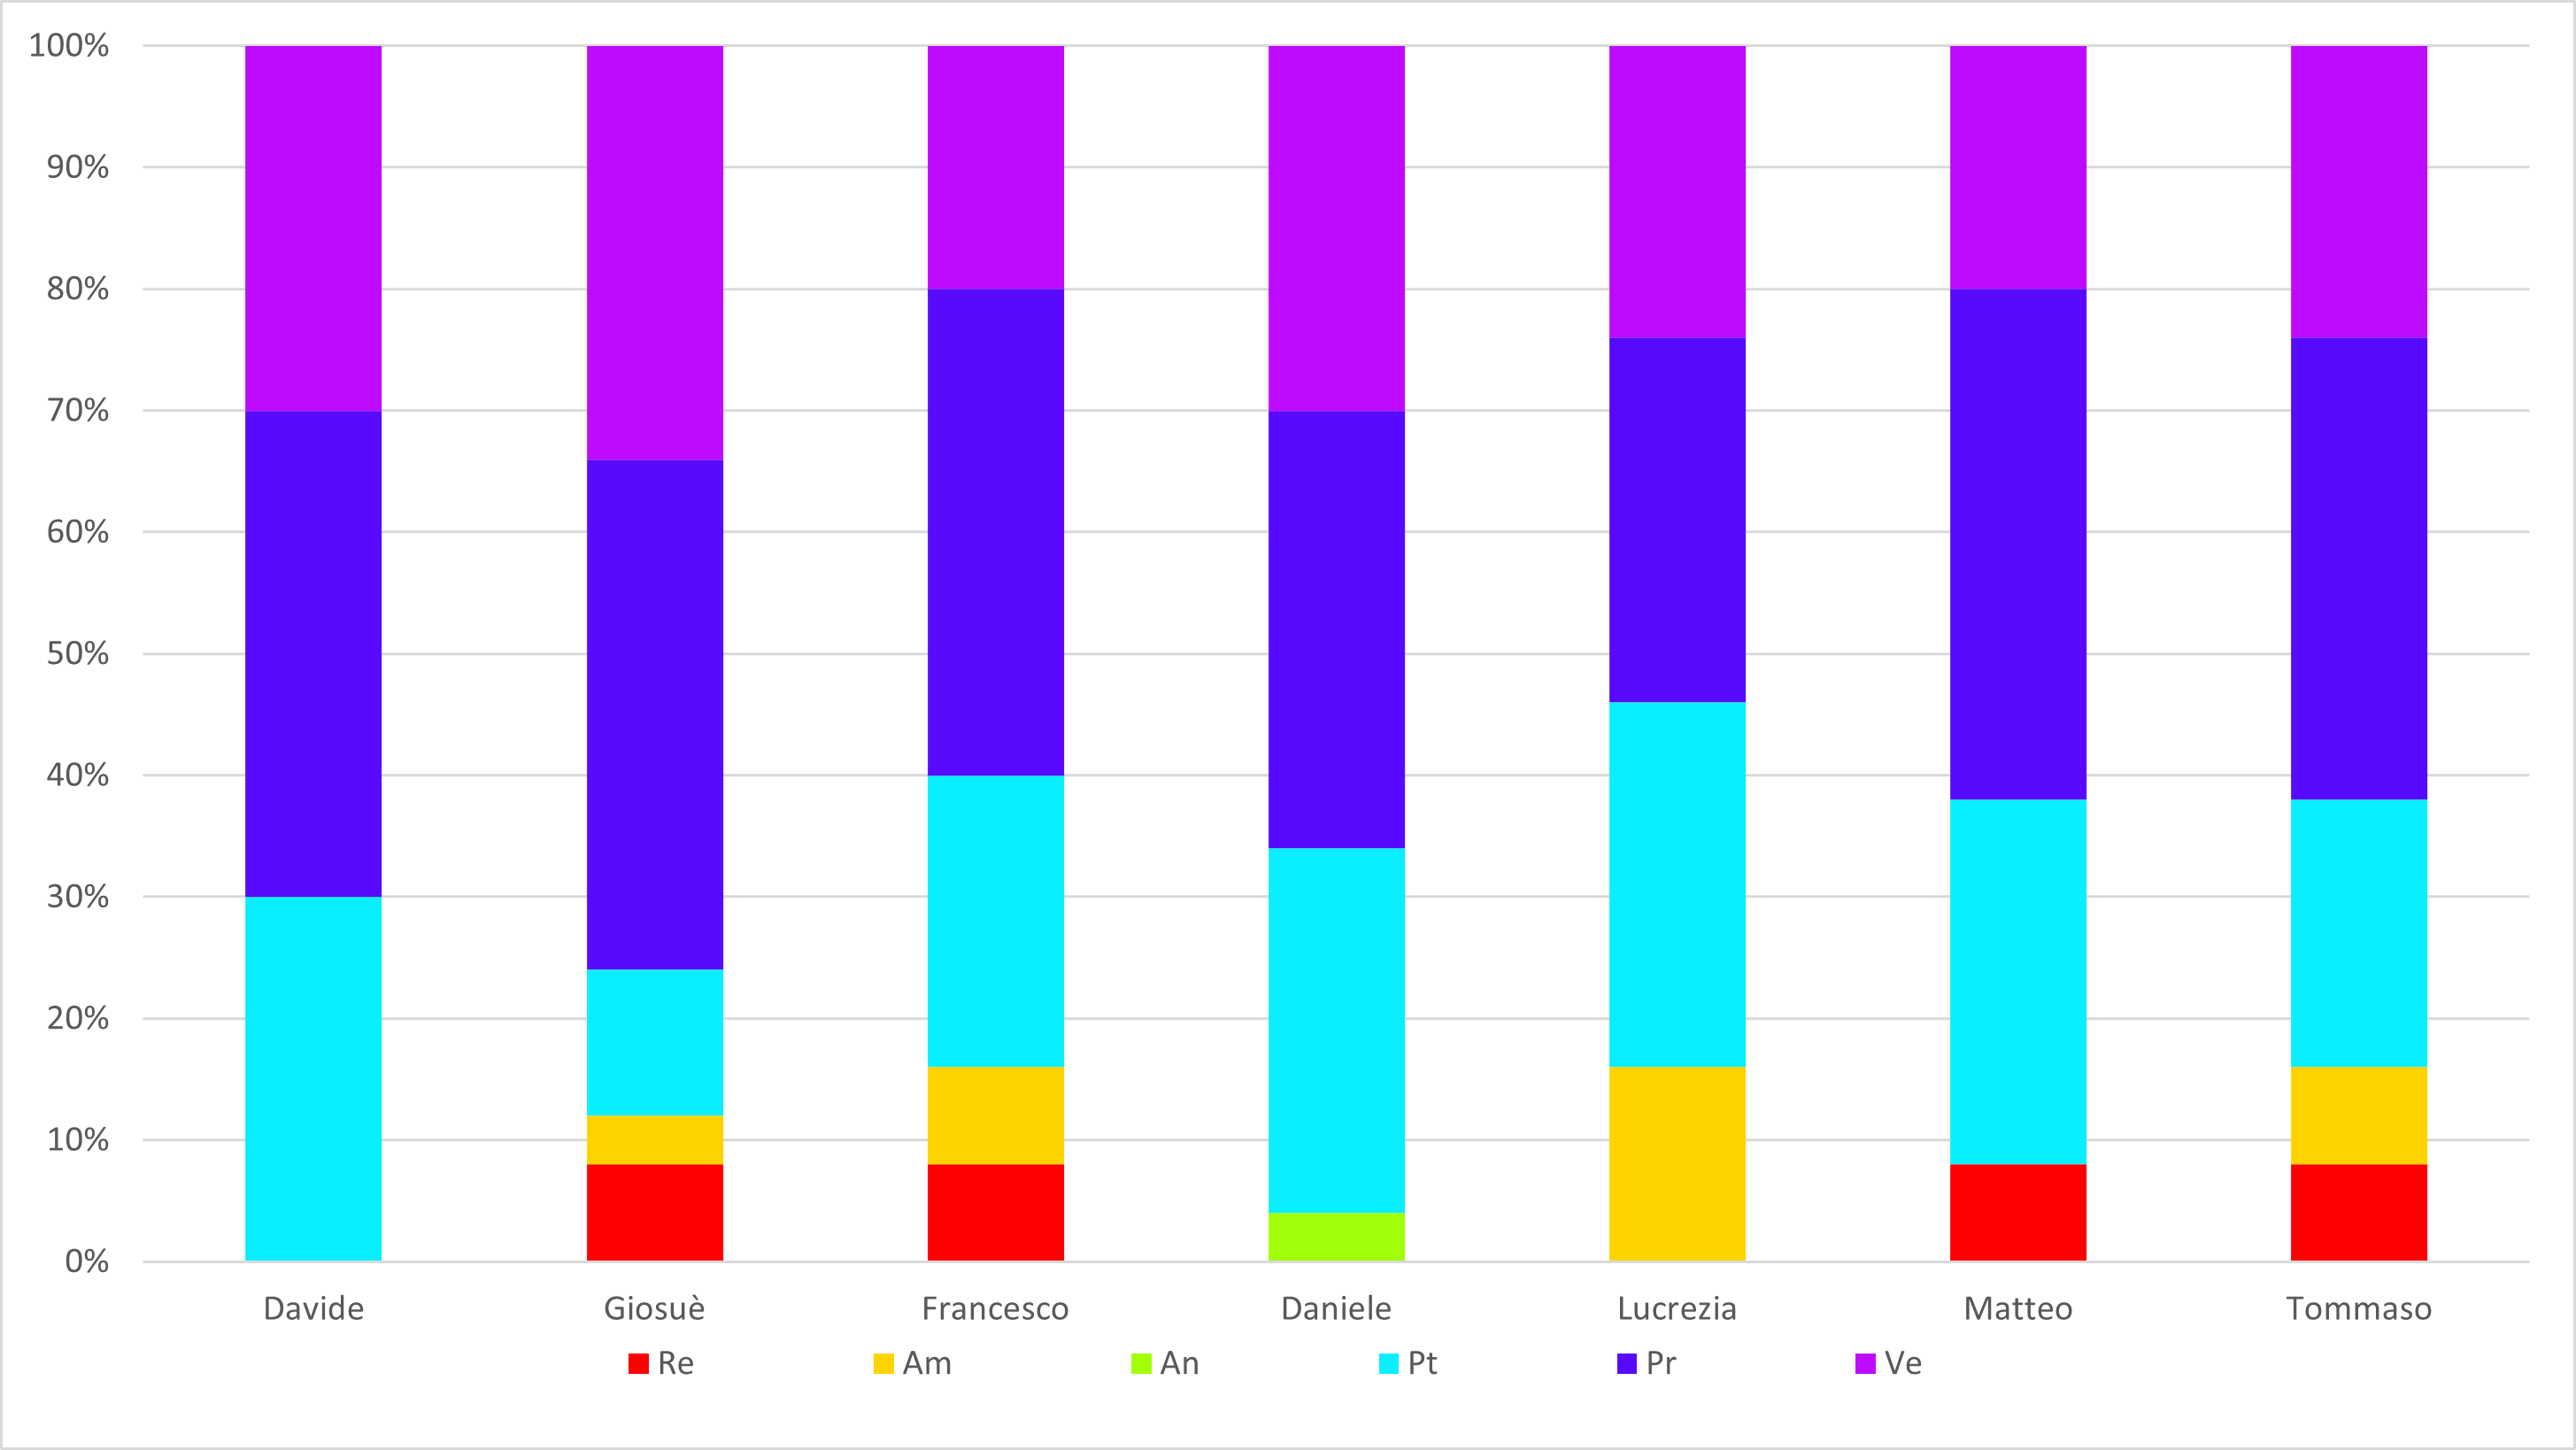
\includegraphics[scale = 0.5]{components/img/Sprint-8-9-isto.png}
    \caption{Istogramma della ripartizione di ore per ruolo in progettazione di dettaglio e codifica}
    \label{fig:Istogramma ripartizione ore , fase di progettazione di dettaglio e codifica}
\end{figure}
\subsubsection{Prospetto economico}
Il costo per ogni ruolo è il seguente:
\begin{table}[H]
		\begin{center}
			\setlength{\aboverulesep}{0pt}
			\setlength{\belowrulesep}{0pt}
			\setlength{\extrarowheight}{.75ex}
			\rowcolors{2}{AzzurroGruppo!10}{white}
			\begin{tabular}{ c c c }
				\rowcolor{AzzurroGruppo!30} 
				\textbf{Ruolo} & \textbf{Ore} & \textbf{Costo}  \\
				\toprule
				Responsabile   & 16 & 480 \euro \\
				Amministratore & 18 & 360 \euro \\
				Analista       & 2 & 50 \euro \\
				Progettista    & 89 & 1958 \euro \\
				Programmatore  & 134 & 2010 \euro \\
				Verificatore   & 91 & 1365 \euro \\
				\textbf{Totale} & \textbf{350} & \textbf{6223 \euro} \\
				\bottomrule
			\end{tabular}
			\caption{ Prospetto dei costi per ruoli nel periodo di progettazione di dettaglio e codifica}
		\end{center}
	\end{table}
I dati ottenuti si possono riassumere nel seguente areogramma:
\begin{figure}[H]
    \centering
    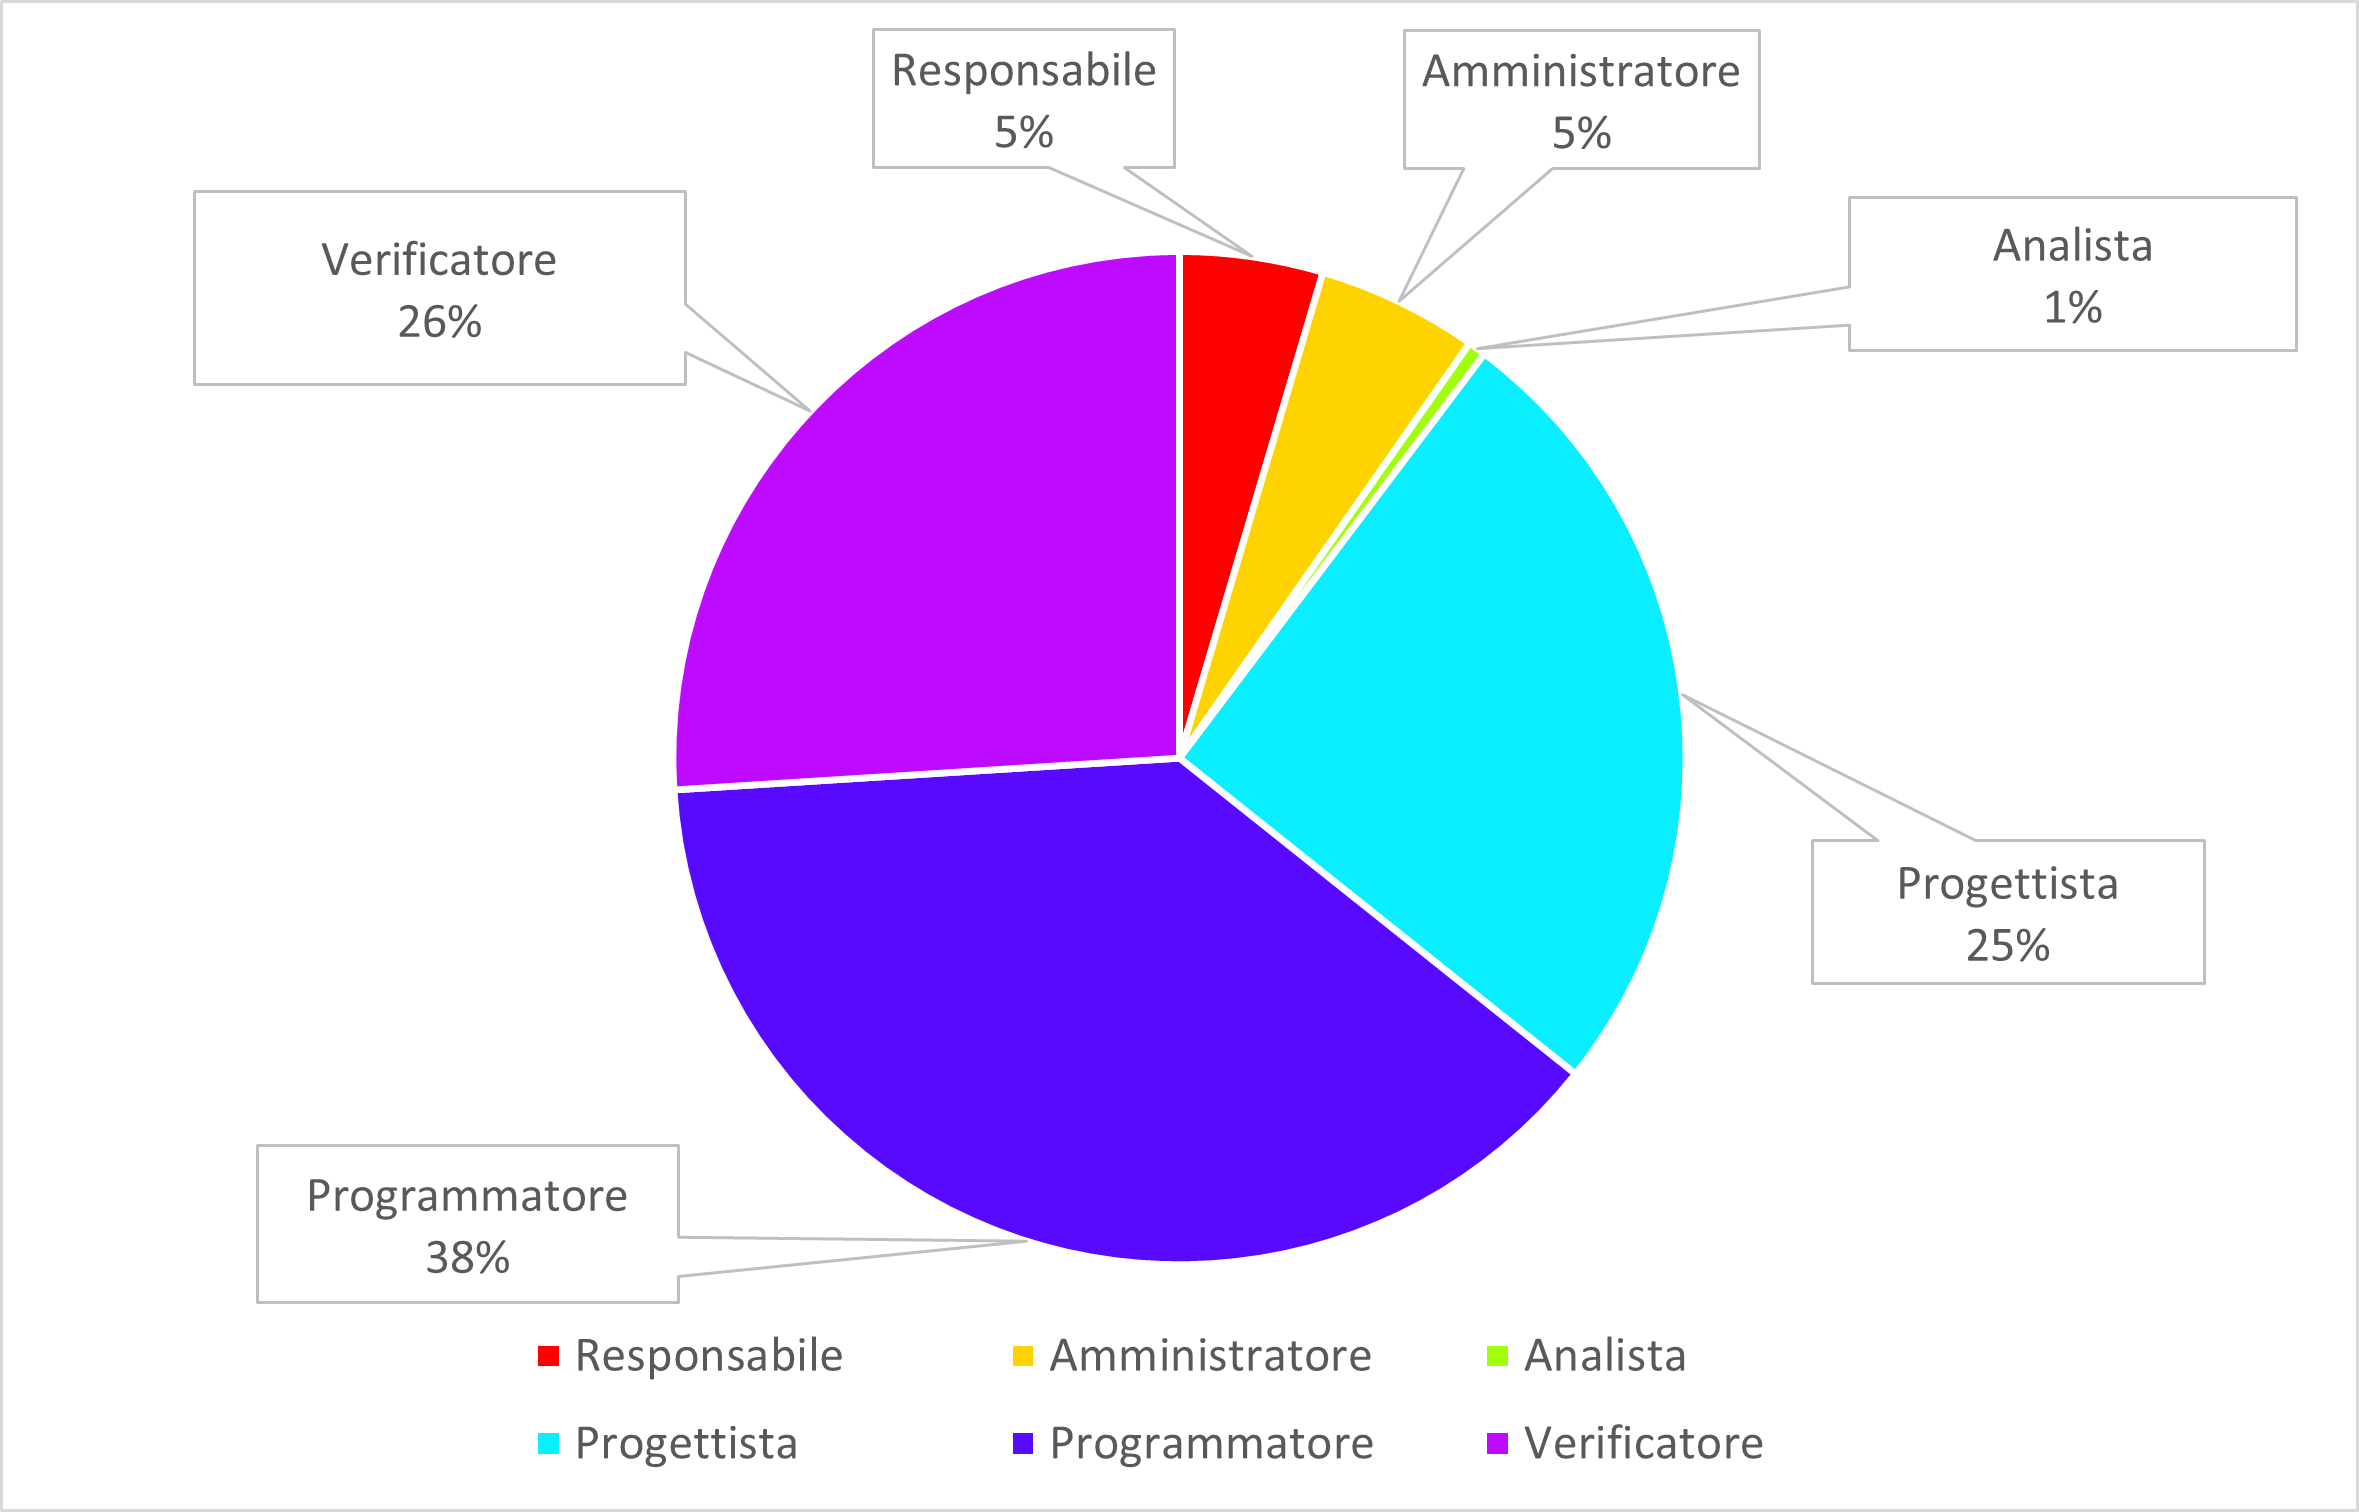
\includegraphics[scale = 0.5]{components/img/Sprint-8-9-torta.png}
    \caption{ Areogramma della ripartizione di ore per ruolo in progettazione di dettaglio e codifica}
    \label{fig:Areogramma ripartizione ore, fase di progettazione di dettaglio e codifica}
\end{figure}
\subsection{Fase di validazione e collaudo}

\subsubsection{Sprint 10}

In questo \glo{sprint} la distribuzione oraria è la seguente:
\begin{table}[H]
		\begin{center}
			\setlength{\aboverulesep}{0pt}
			\setlength{\belowrulesep}{0pt}
			\setlength{\extrarowheight}{.75ex}
			\rowcolors{2}{AzzurroGruppo!10}{white}
			\begin{tabular}{ c c c c c c c c }
				\rowcolor{AzzurroGruppo!30} 
				\textbf{Nominativo} & \textbf{Re} & \textbf{Am} & \textbf{An} & \textbf{Pt} & \textbf{Pr} & \textbf{Ve} & \textbf{Ore Totali}  \\
				\toprule
				\Davide    & 2 & 3 & - & - & - & 2 & 7 \\
				\Giosue    & - & - & - & 2 & 3 & 2 & 7 \\
				\Francesco & - & 3 & - & - & 3 & 2 & 8\\
				\Daniele   & 4 & - & - & - & 2 & - & 6\\
				\Lucrezia  & - & - & - & - & 4 & 3 & 7\\
				\Matteo    & - & - & - & - & - & 7 & 7\\
				\Tommaso   & - & - & - & 2 & - & 5 & 7\\
				 \textbf{Ore totali} & \textbf{6} & \textbf{6} & \textbf{-} & \textbf{4} & \textbf{12} & \textbf{21} & \textbf{49} \\
				\bottomrule
			\end{tabular}
			\caption{Distribuzione delle ore nello sprint 10}
		\end{center}
	\end{table}


\subsubsection{Sprint 11}


In questo \glo{sprint} la distribuzione oraria è la seguente:
\begin{table}[H]
		\begin{center}
			\setlength{\aboverulesep}{0pt}
			\setlength{\belowrulesep}{0pt}
			\setlength{\extrarowheight}{.75ex}
			\rowcolors{2}{AzzurroGruppo!10}{white}
			\begin{tabular}{ c c c c c c c c }
				\rowcolor{AzzurroGruppo!30} 
				\textbf{Nominativo} & \textbf{Re} & \textbf{Am} & \textbf{An} & \textbf{Pt} & \textbf{Pr} & \textbf{Ve} & \textbf{Ore Totali}  \\
				\toprule
				\Davide    & - & - & - & - & 5 & 2 & 7 \\
				\Giosue    & - & - & - & 2 & 3 & 2 & 7 \\
				\Francesco & - & 3 & - & - & 3 & - & 6\\
				\Daniele   & 2 & - & - & - & - & 4 & 6\\
				\Lucrezia  & 5 & - & - & - & - & 2 & 7\\
				\Matteo    & - & - & - & - & 3 & 3 & 6\\
				\Tommaso   & - & 3 & - & - & - & 3 & 6\\
				 \textbf{Ore totali} & \textbf{7} & \textbf{6} & \textbf{-} & \textbf{2} & \textbf{14} & \textbf{16} & \textbf{45} \\
				\bottomrule
			\end{tabular}
			\caption{Distribuzione delle ore nello sprint 11}
		\end{center}
	\end{table}
	
\subsubsection{Sprint 12}
In questo \glo{sprint} la distribuzione oraria è la seguente:
\begin{table}[H]
		\begin{center}
			\setlength{\aboverulesep}{0pt}
			\setlength{\belowrulesep}{0pt}
			\setlength{\extrarowheight}{.75ex}
			\rowcolors{2}{AzzurroGruppo!10}{white}
			\begin{tabular}{ c c c c c c c c }
				\rowcolor{AzzurroGruppo!30} 
				\textbf{Nominativo} & \textbf{Re} & \textbf{Am} & \textbf{An} & \textbf{Pt} & \textbf{Pr} & \textbf{Ve} & \textbf{Ore Totali}  \\
				\toprule
				\Davide    & 2 & 2 & - & - & - & 2 & 6 \\
				\Giosue    & - & - & - & - & - & 6 & 6 \\
				\Francesco & - & - & - & - & 2 & 4 & 6\\
				\Daniele   & 2 & - & - & - & 2 & 4 & 8\\
				\Lucrezia  & - & - & - & - & 3 & 3 & 6\\
				\Matteo    & - & - & - & - & 3 & 4 & 7\\
				\Tommaso   & - & 2 & - & 3 & - & 2 & 7\\
				 \textbf{Ore totali} & \textbf{4} & \textbf{4} & \textbf{-} & \textbf{3} & \textbf{10} & \textbf{25} & \textbf{46} \\
				\bottomrule
			\end{tabular}
			\caption{Distribuzione delle ore nello sprint 12}
		\end{center}
	\end{table}


\subsubsection{Prospetto orario}
In questa fase la distribuzione oraria è la seguente:
\begin{table}[H]
		\begin{center}
			\setlength{\aboverulesep}{0pt}
			\setlength{\belowrulesep}{0pt}
			\setlength{\extrarowheight}{.75ex}
			\rowcolors{2}{AzzurroGruppo!10}{white}
			\begin{tabular}{ c c c c c c c c }
				\rowcolor{AzzurroGruppo!30} 
				\textbf{Nominativo} & \textbf{Re} & \textbf{Am} & \textbf{An} & \textbf{Pt} & \textbf{Pr} & \textbf{Ve} & \textbf{Ore Totali}  \\
				\toprule
				\Davide    & 4 & 5 & - & - & 5 & 6 & 20 \\
				\Giosue    & - & - & - & 4 & 6 & 10 & 20 \\
				\Francesco & - & 6 & - & - & 8 & 6 & 20\\
				\Daniele   & 8 & - & - & - & 4 & 8 & 20\\
				\Lucrezia  & 5 & - & - & - & 7 & 8 & 20\\
				\Matteo    & - & - & - & - & 6 & 14 & 20\\
				\Tommaso   & - & 5 & - & 5 & - & 10 & 20\\
				 \textbf{Ore totali} & \textbf{17} & \textbf{16} & \textbf{-} & \textbf{9} & \textbf{36} & \textbf{62} & \textbf{140} \\
				\bottomrule
			\end{tabular}
			\caption{Distribuzione delle ore nel periodo di validazione e collaudo}
		\end{center}
	\end{table}
	I dati ottenuti vengono riassunti nel seguente istogramma:
	\begin{figure}[H]
    \centering
    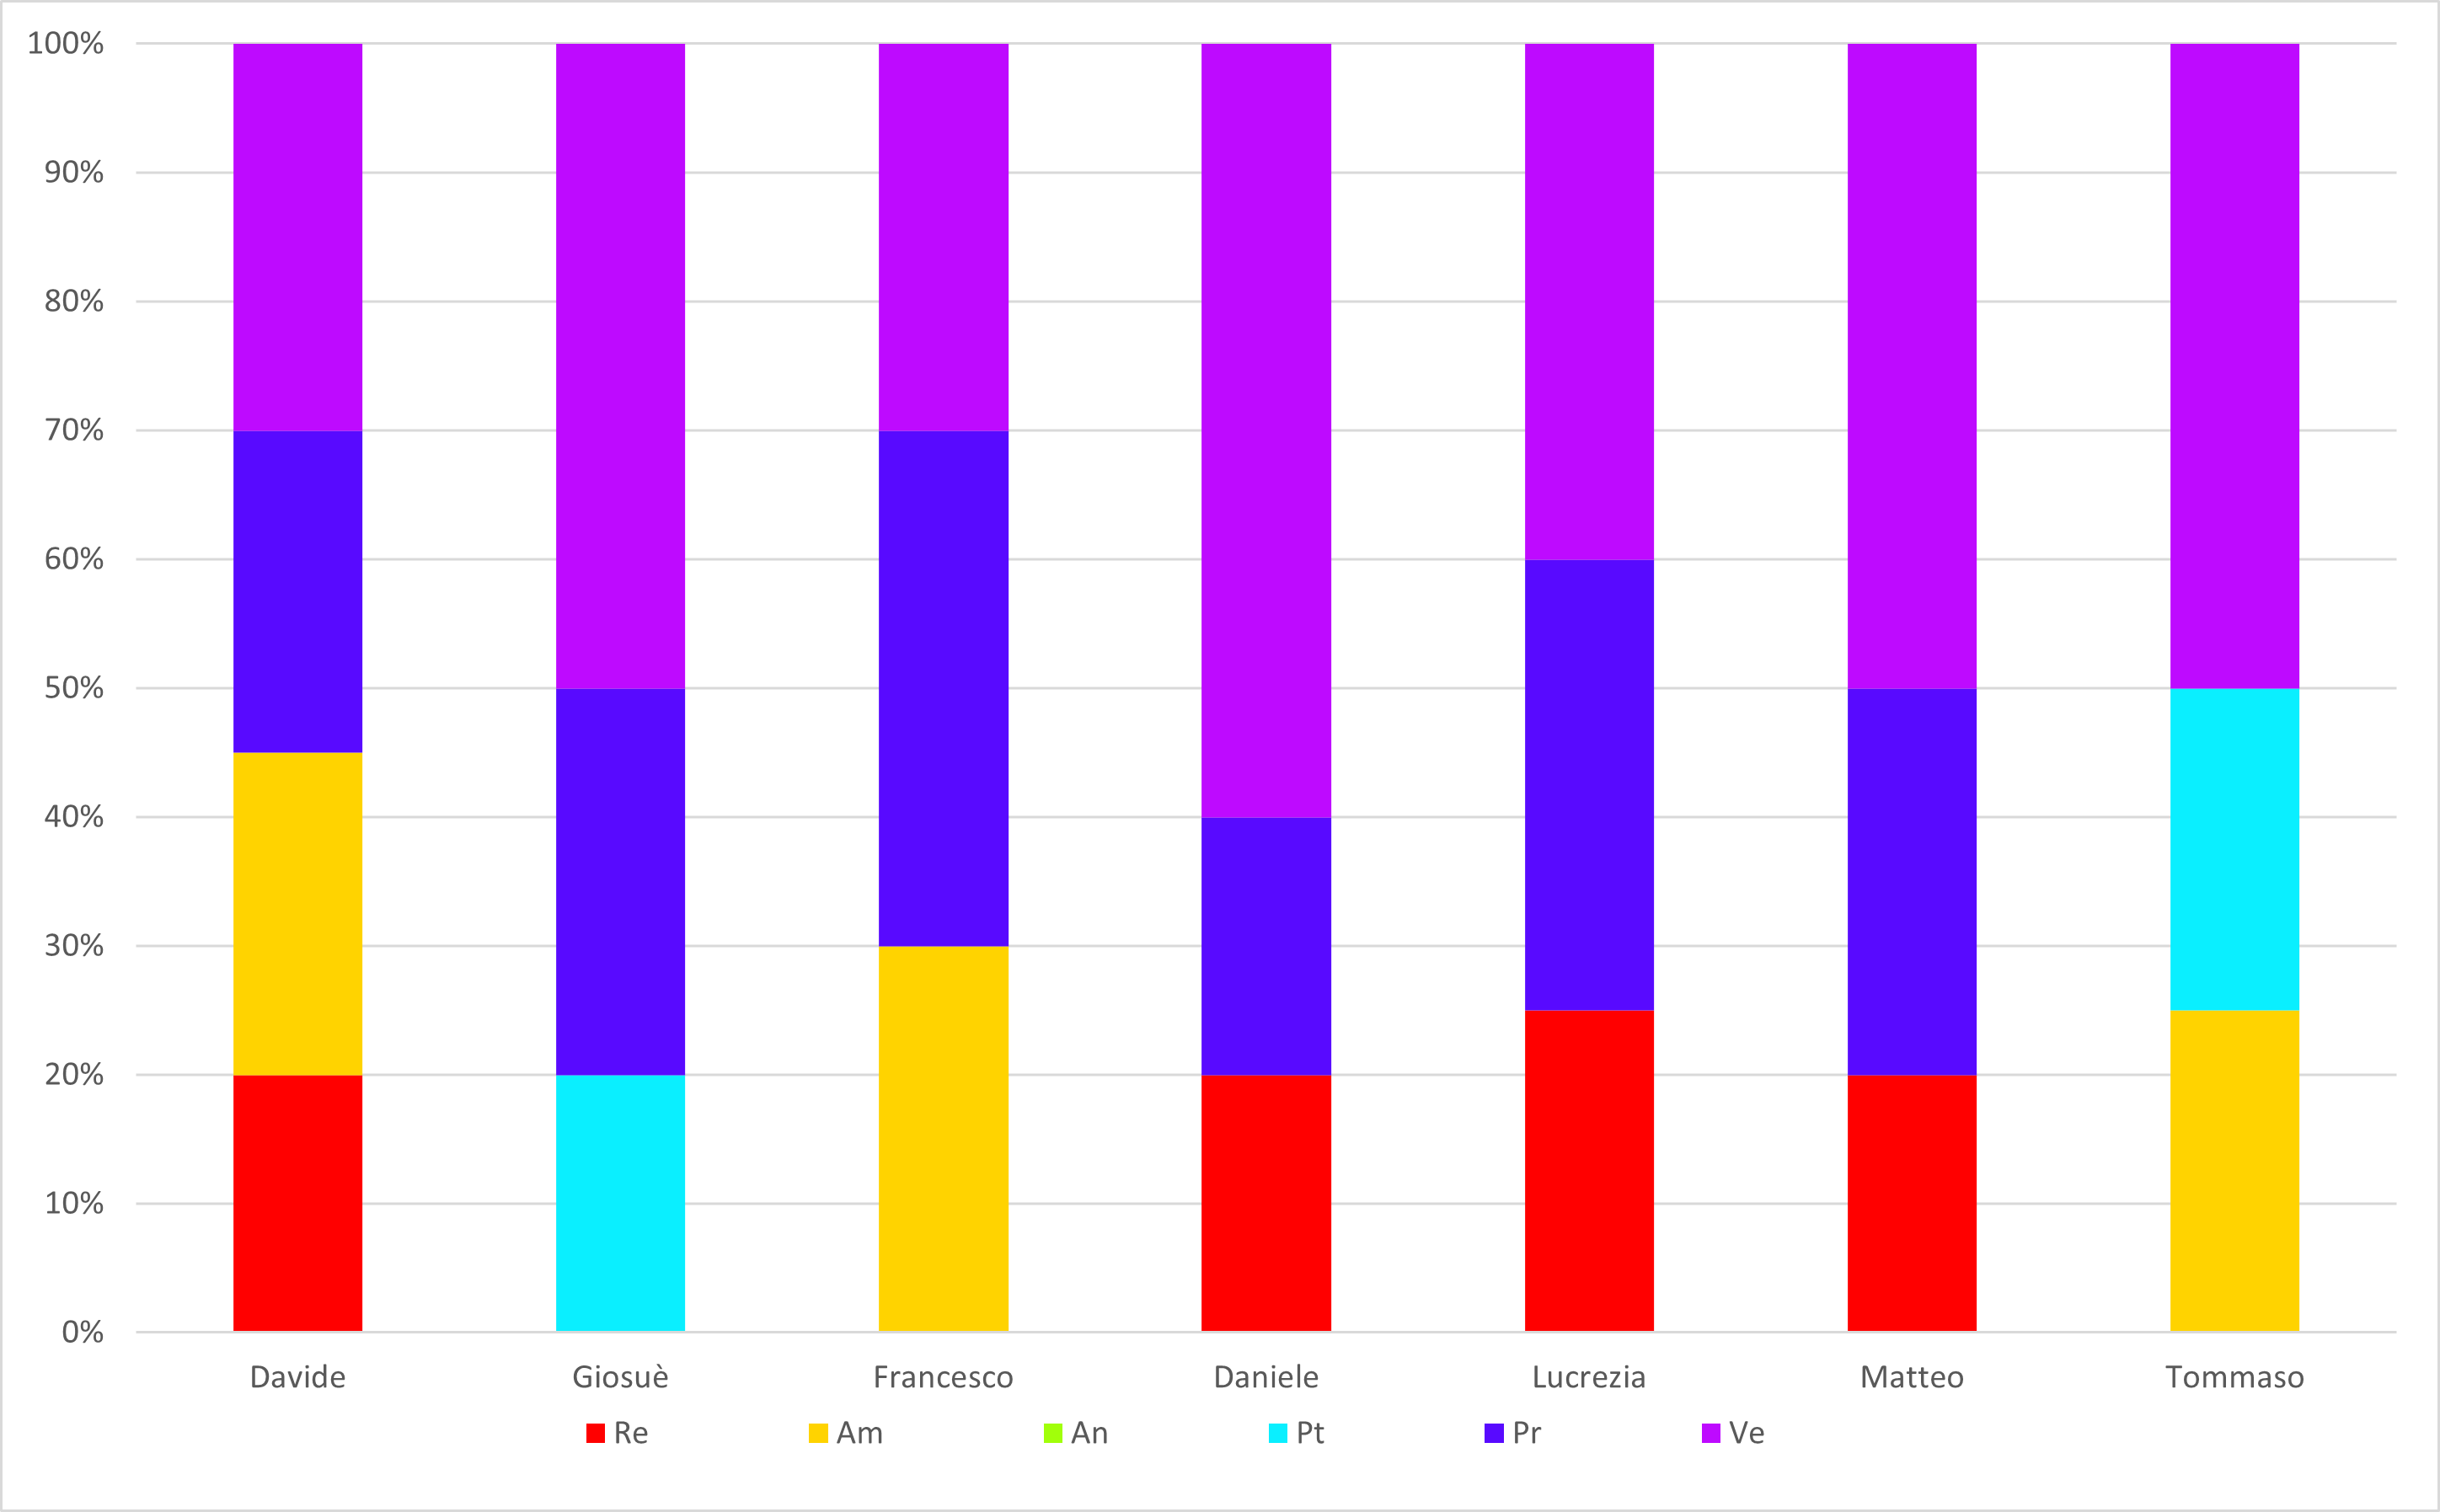
\includegraphics[scale = 0.5]{components/img/Sprint-10-11-isto.png}
    \caption{Istogramma della ripartizione di ore per ruolo in validazione e collaudo}
    \label{fig:Istogramma ripartizione ore , fase di validazione e collaudo}
\end{figure}
\subsubsection{Prospetto economico}
Il costo per ogni ruolo è il seguente:
\begin{table}[H]
		\begin{center}
			\setlength{\aboverulesep}{0pt}
			\setlength{\belowrulesep}{0pt}
			\setlength{\extrarowheight}{.75ex}
			\rowcolors{2}{AzzurroGruppo!10}{white}
			\begin{tabular}{ c c c }
				\rowcolor{AzzurroGruppo!30} 
				\textbf{Ruolo} & \textbf{Ore} & \textbf{Costo}  \\
				\toprule
				Responsabile   & 17 & 510 \euro \\
				Amministratore & 16 & 320 \euro \\
				Analista       & -  & - \\
				Progettista    & 9  & 198 \euro \\
				Programmatore  & 36 & 540 \euro \\
				Verificatore   & 62 & 930 \euro \\
				\textbf{Totale} & \textbf{140} & \textbf{2498 \euro} \\
				\bottomrule
			\end{tabular}
			\caption{ Prospetto dei costi per ruoli nel periodo di validazione e collaudo}
		\end{center}
	\end{table}
I dati ottenuti si possono riassumere nel seguente areogramma:
\begin{figure}[H]
    \centering
    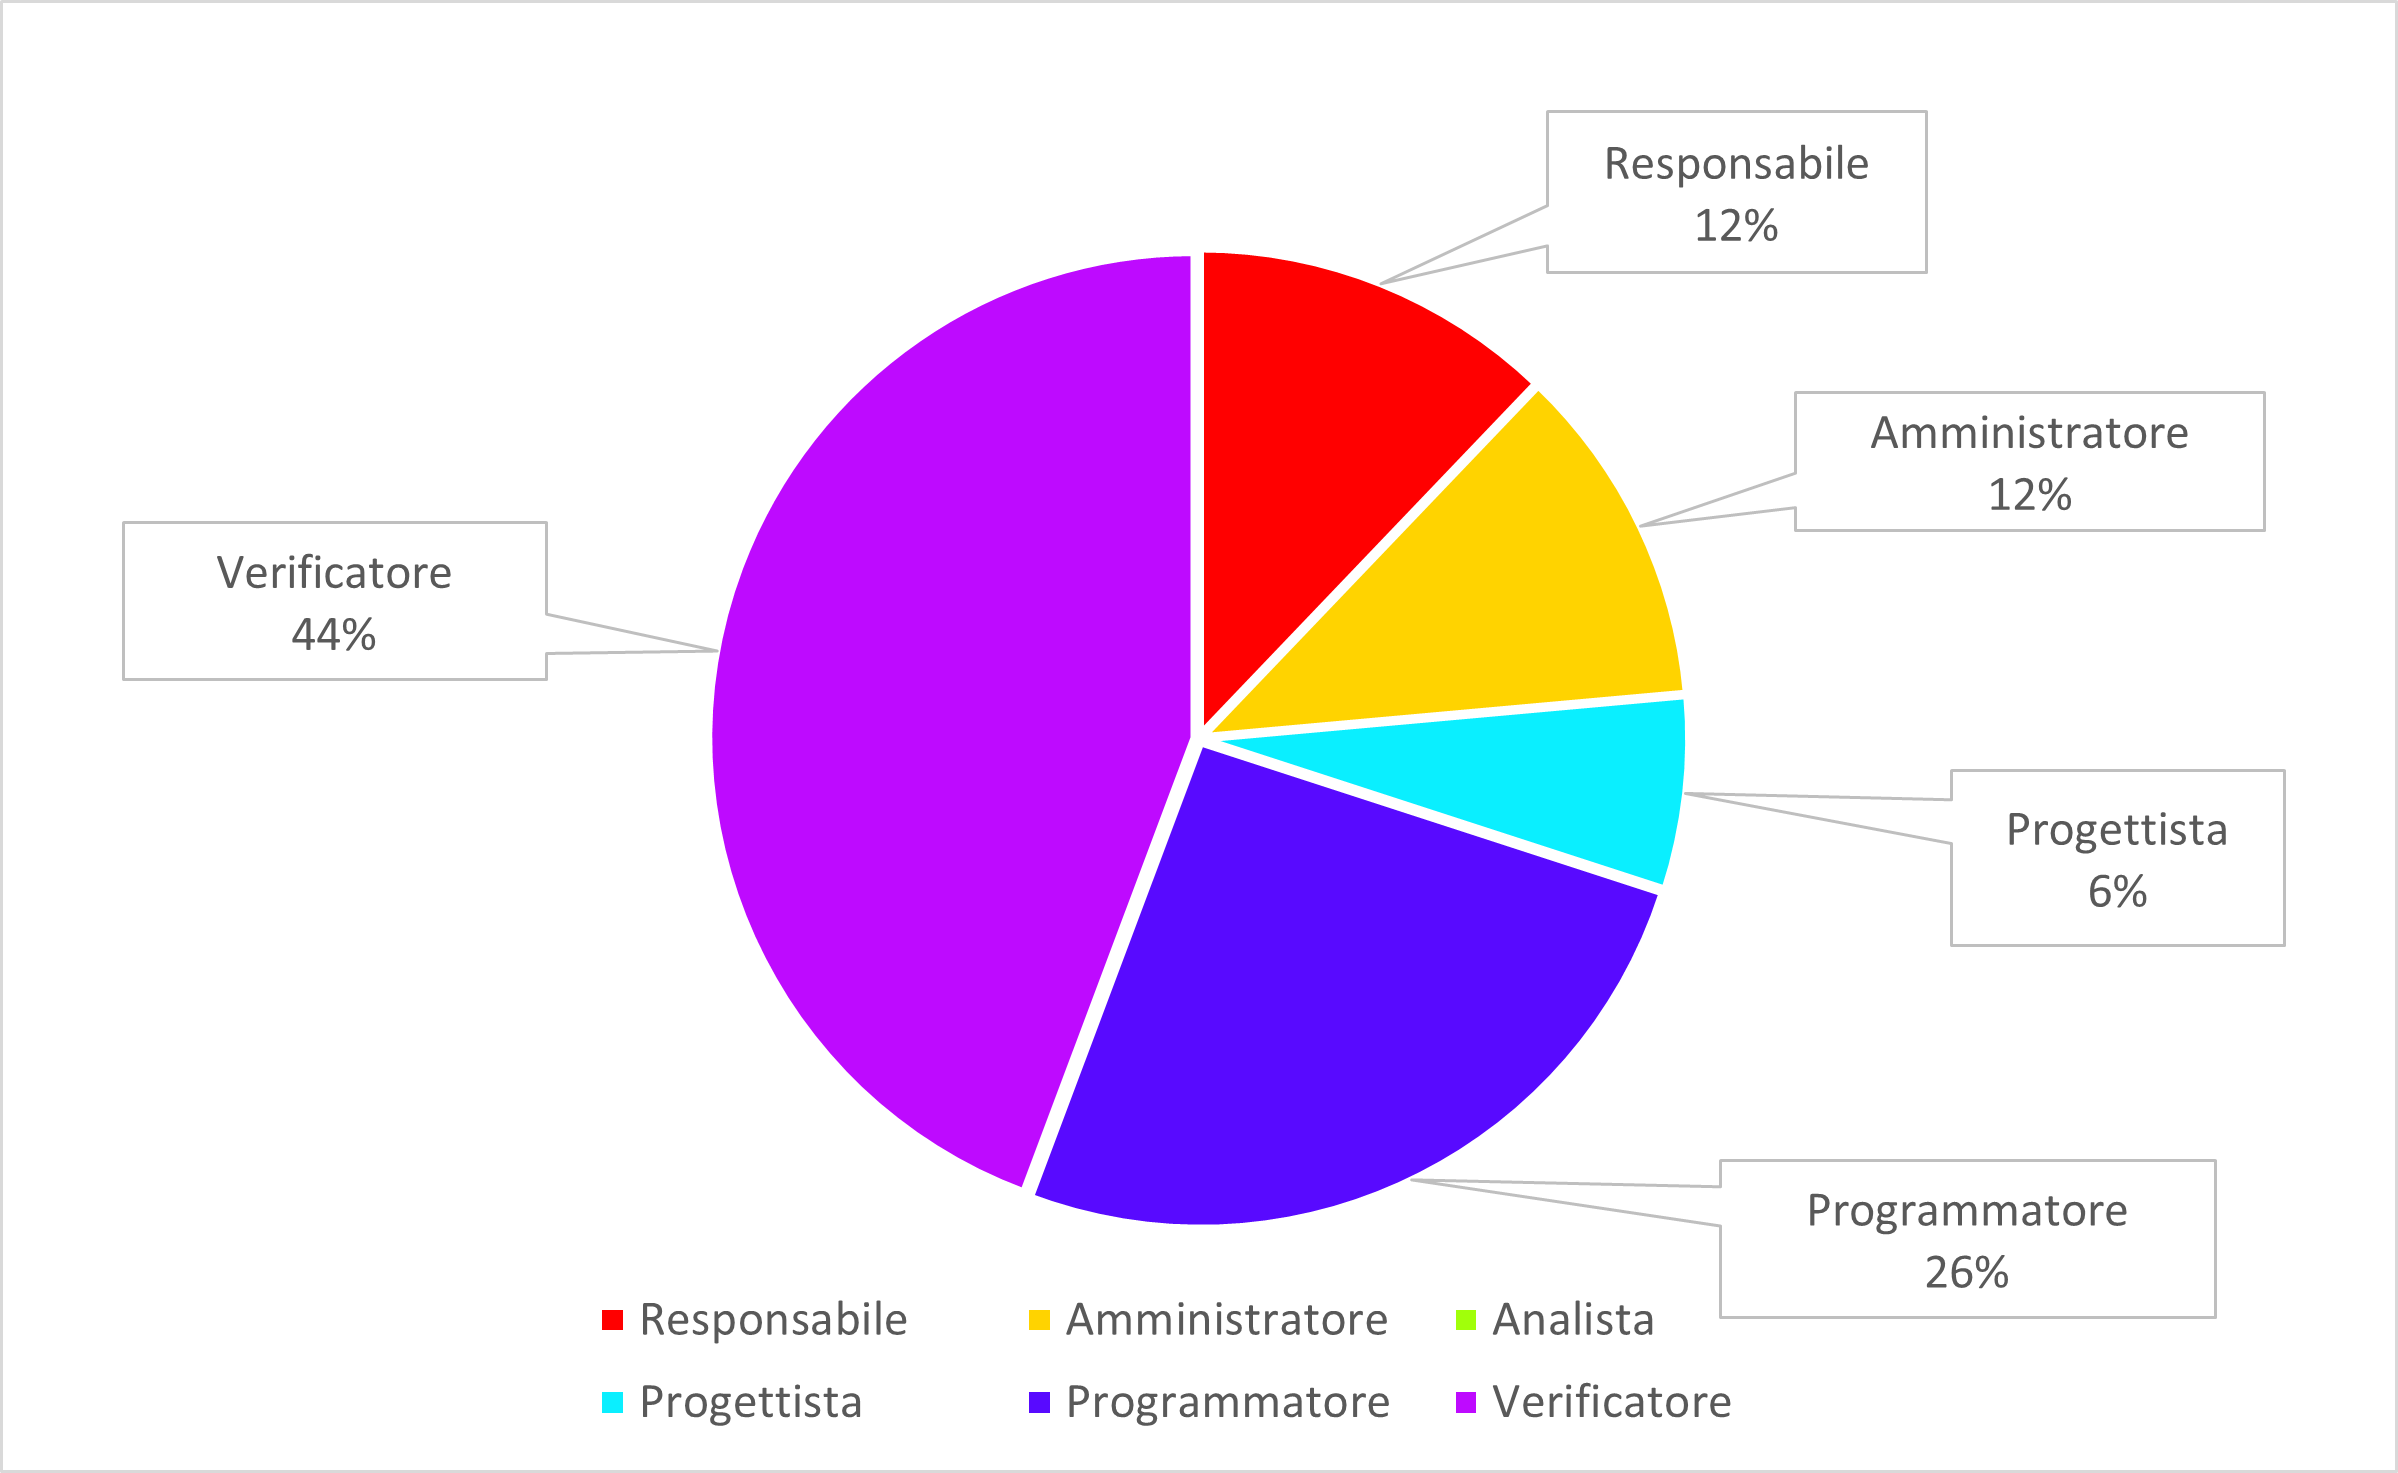
\includegraphics[scale = 0.5]{components/img/Sprint-10-11-torta.png}
    \caption{ Areogramma della ripartizione di ore per ruolo in validazione e collaudo}
    \label{fig:Areogramma ripartizione ore , fase di validazione e collaudo}
\end{figure}
\subsection{Riepilogo}
\subsubsection{Ore totali}
\paragraph{Suddivisione del lavoro}
Nella seguente tabella vengono riportate il totale delle ore del progetto, sono presenti sia le ore di investimento, sia le ore rendicontate a carico del committente.
\begin{table}[H]
		\begin{center}
			\setlength{\aboverulesep}{0pt}
			\setlength{\belowrulesep}{0pt}
			\setlength{\extrarowheight}{.75ex}
			\rowcolors{2}{AzzurroGruppo!10}{white}
			\begin{tabular}{ c c c c c c c c }
				\rowcolor{AzzurroGruppo!30} 
				\textbf{Nominativo} & \textbf{Re} & \textbf{Am} & \textbf{An} & \textbf{Pt} & \textbf{Pr} & \textbf{Ve} & \textbf{Ore Totali}  \\
				\toprule
				\Davide    & 9 & 16 & 18 & 15 & 29 & 48 & 135 \\
				\Giosue    & 7 & 10 & 17 & 26 & 32 & 43 & 135 \\
				\Francesco & 13 & 14 & 23 & 24 & 31 & 30 & 135\\
				\Daniele   & 18 & 6 & 22 & 28 & 22 & 43 & 135\\
				\Lucrezia  & 18 & 11 & 17 & 15 & 26 & 48 & 135\\
				\Matteo    & 14 & 13 & 17 & 27 & 27 & 33 & 135\\
				\Tommaso   & 4 & 19 & 26 & 24 & 24 & 38 & 135\\
				 \textbf{Ore totali} & \textbf{83} & \textbf{89} & \textbf{140} & \textbf{159} & \textbf{191} & \textbf{283} & \textbf{945} \\
				\bottomrule
			\end{tabular}
			\caption{ Distribuzione delle ore totali di investimento e rendicontate}
		\end{center}
	\end{table}
	I dati ottenuti vengono riassunti nel seguente istogramma:
\begin{figure}[H]
    \centering
    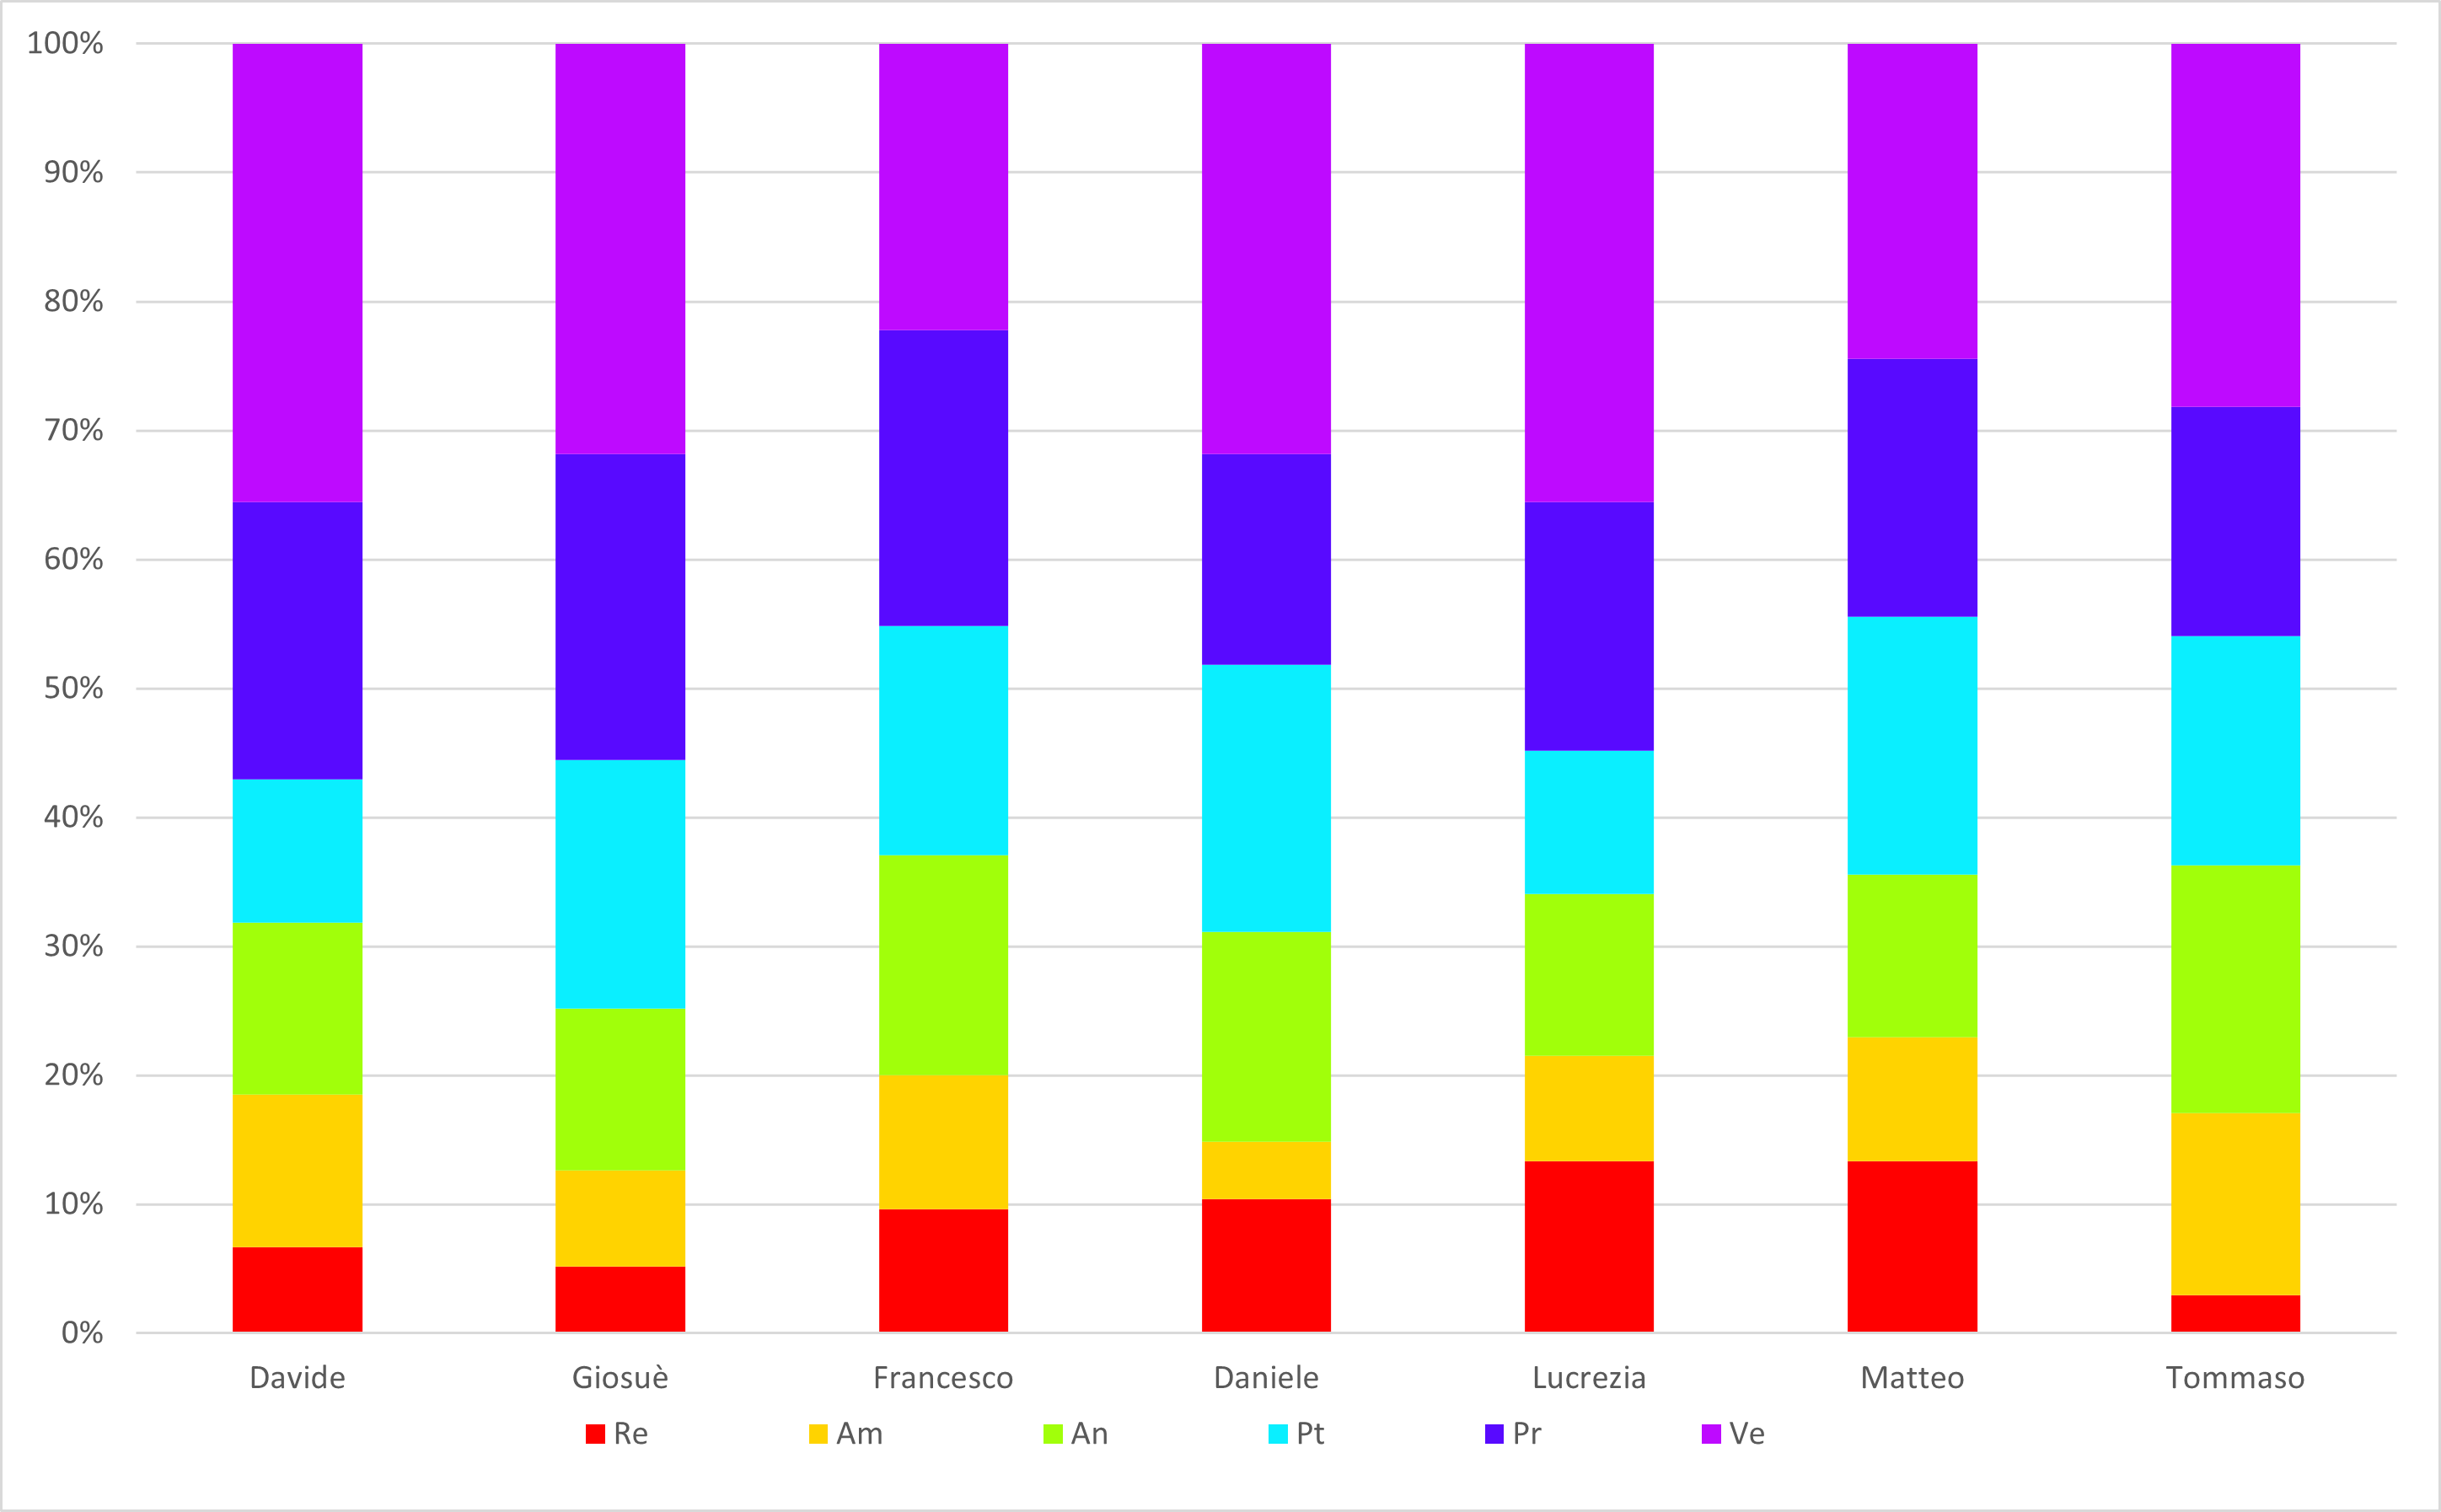
\includegraphics[scale = 0.5]{components/img/Totale-non-rendicontate-isto.png}
    \caption{ Istogramma della ripartizione di ore totali di investimento e rendicontate}
    \label{fig:Istogramma ripartizione ore totali di investimento e rendicontate }
\end{figure}
\paragraph{Prospetto economico}
Il costo per ogni ruolo è il seguente:
\begin{table}[H]
		\begin{center}
			\setlength{\aboverulesep}{0pt}
			\setlength{\belowrulesep}{0pt}
			\setlength{\extrarowheight}{.75ex}
			\rowcolors{2}{AzzurroGruppo!10}{white}
			\begin{tabular}{ c c c }
				\rowcolor{AzzurroGruppo!30} 
				\textbf{Ruolo} & \textbf{Ore} & \textbf{Costo}  \\
				\toprule
				Responsabile   & 83 & 2490 \euro \\
				Amministratore & 89 & 1780 \euro \\
				Analista       & 140 & 3500 \euro \\
				Progettista    & 159 & 3498 \euro \\
				Programmatore  & 191 & 2865 \euro \\
				Verificatore   & 283 & 4245 \euro \\
				\textbf{Totale} & \textbf{945} & \textbf{18378 \euro} \\
				\bottomrule
			\end{tabular}
			\caption{ Prospetto dei costi totale delle ore di investimento e rendicontate}
		\end{center}
	\end{table}
I dati ottenuti si possono riassumere nel seguente areogramma:
\begin{figure}[H]
    \centering
    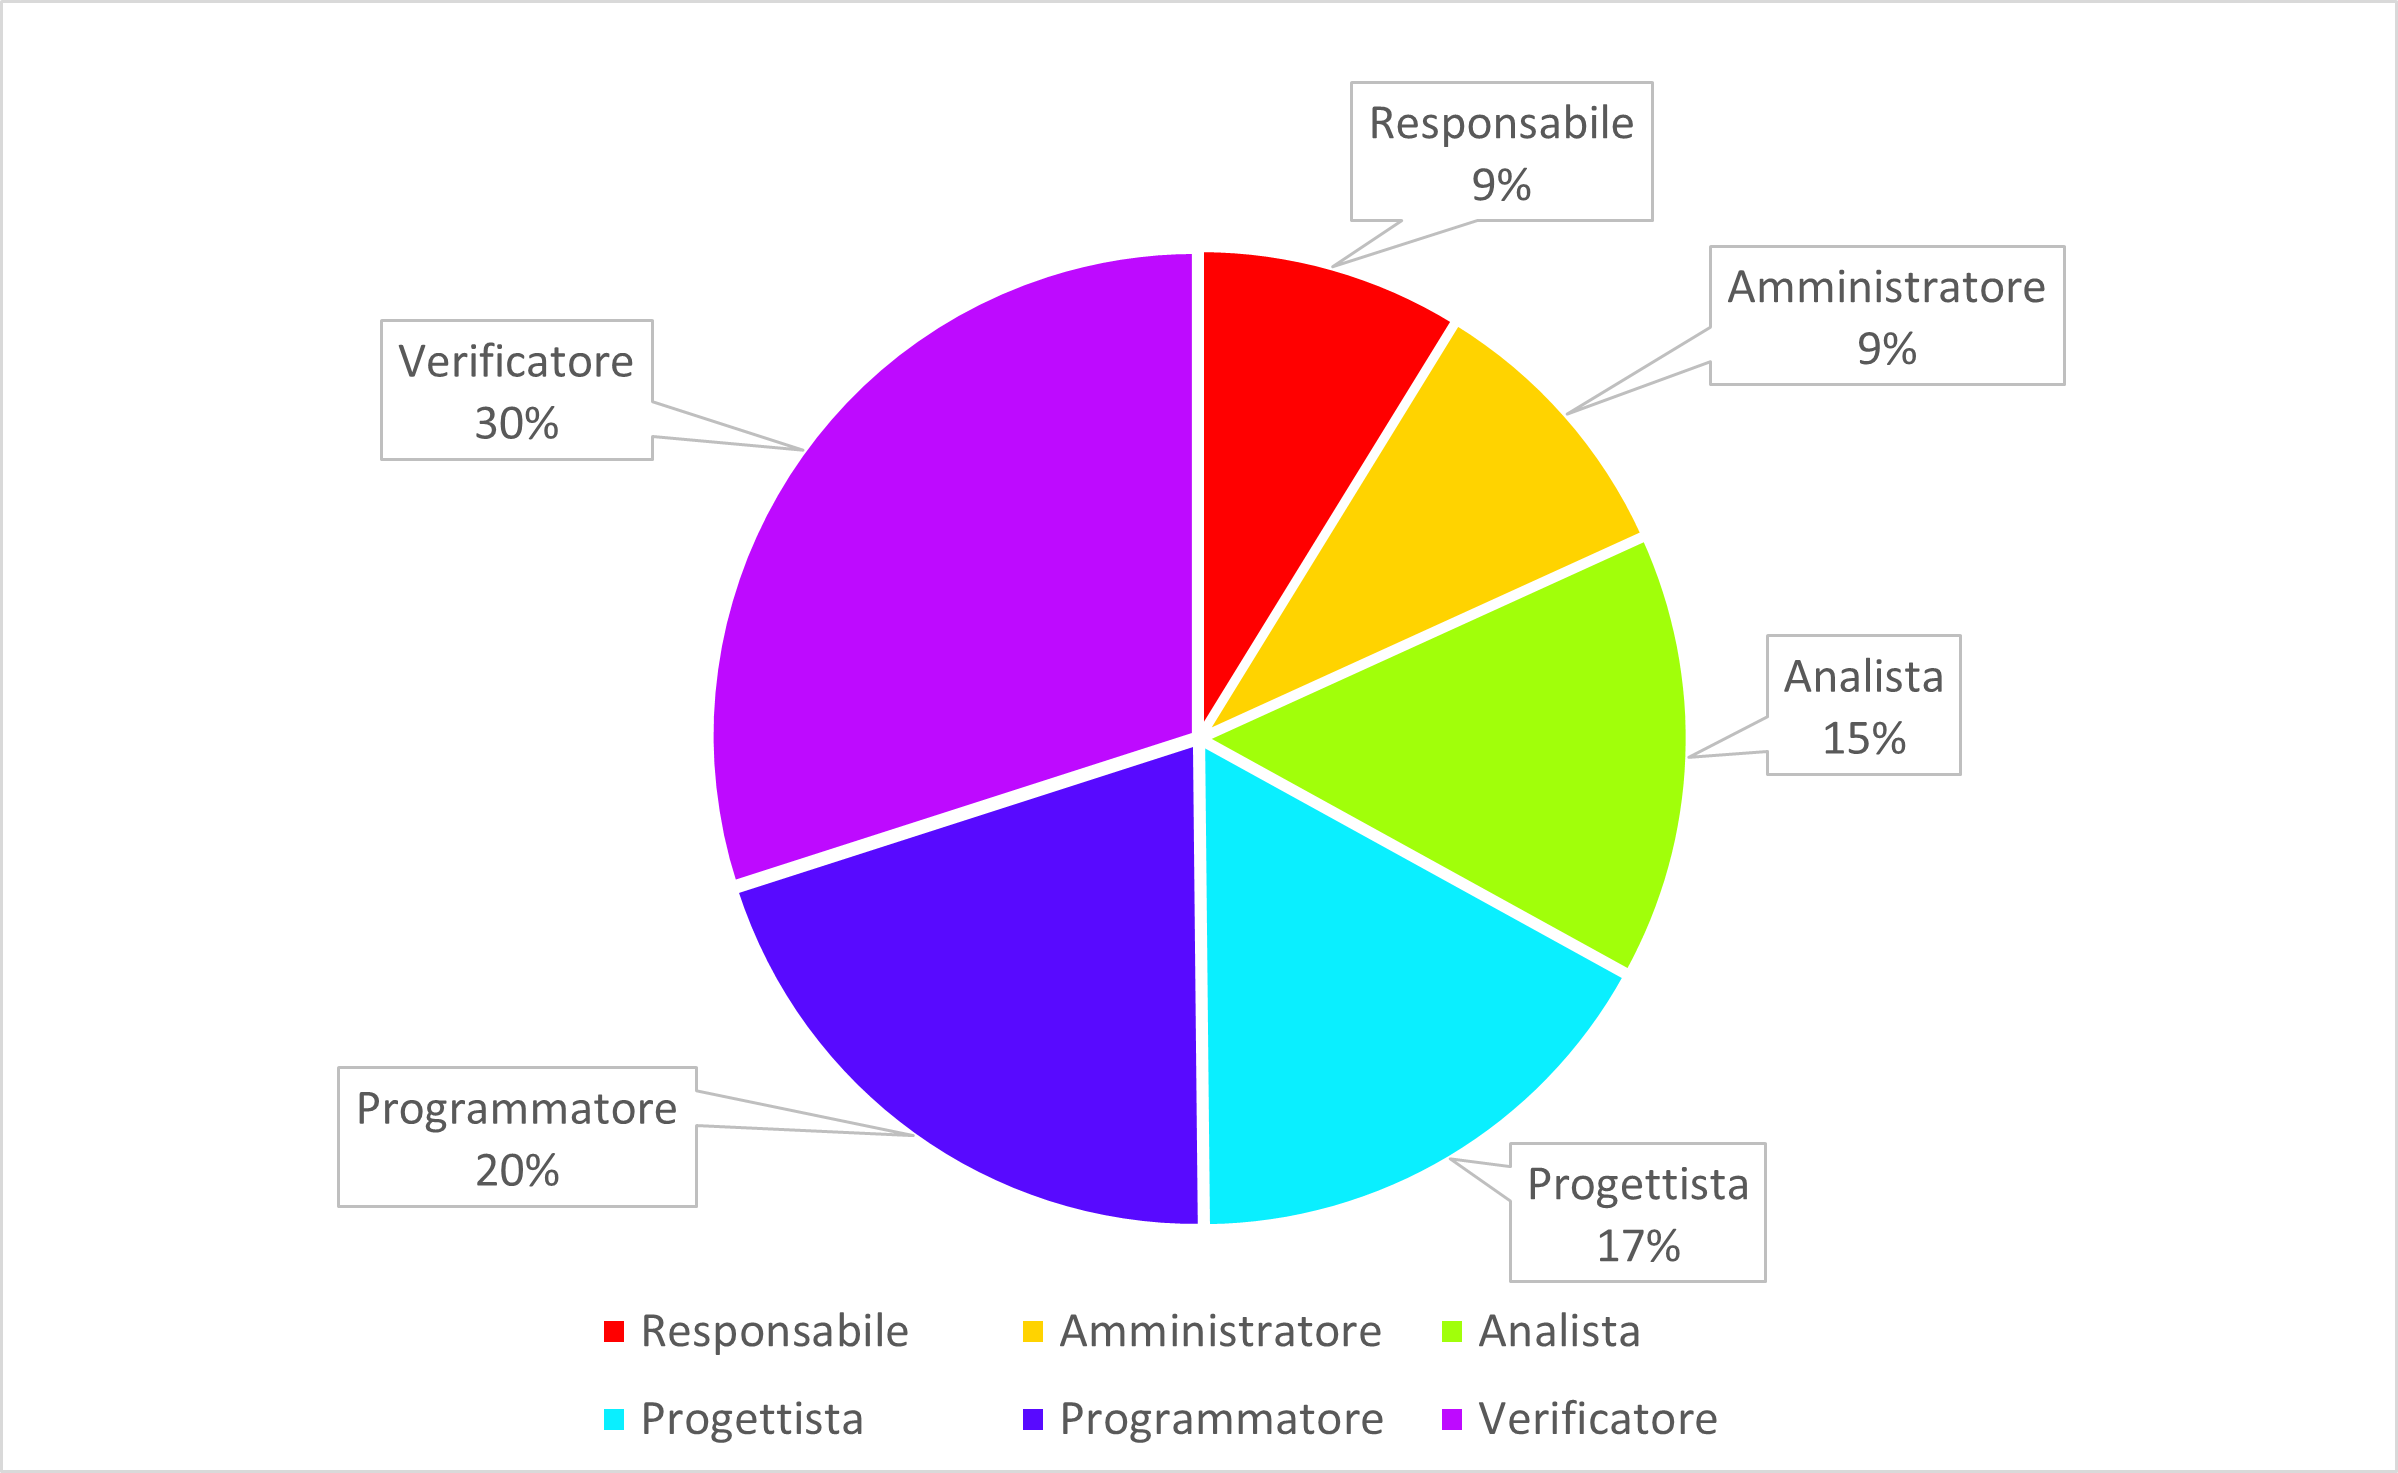
\includegraphics[scale = 0.5]{components/img/Totale-non-rendicontate-torta.png}
    \caption{ Areogramma dei costi totale delle ore di investimento e rendicontate}
    \label{fig:Areogramma ripartizione ore totali di investimento e rendicontate}
\end{figure}
\subsubsection{Ore rendicontate}
\paragraph{Suddivisione del lavoro}
Nella seguente tabella sono riassunte le ore rendicontate:
\begin{table}[H]
		\begin{center}
			\setlength{\aboverulesep}{0pt}
			\setlength{\belowrulesep}{0pt}
			\setlength{\extrarowheight}{.75ex}
			\rowcolors{2}{AzzurroGruppo!10}{white}
			\begin{tabular}{ c c c c c c c c }
				\rowcolor{AzzurroGruppo!30} 
				\textbf{Nominativo} & \textbf{Re} & \textbf{Am} & \textbf{An} & \textbf{Pt} & \textbf{Pr} & \textbf{Ve} & \textbf{Ore Totali}  \\
				\toprule
				\Davide    & 9  & 11 & -  & 15  & 29 & 36 & 100 \\
				\Giosue    & 7  & 2 & -  & 26 & 32 & 33  & 100 \\
				\Francesco & 4  & 10 & 8  & 24 & 31 & 23  & 100\\
				\Daniele   & 8  & 3 & 11 & 28 & 22 & 31  & 100\\
				\Lucrezia  & 5  & 8 & 10 & 15  & 26 & 36 & 100\\
				\Matteo    & 14 & 8 & -  & 27 & 27 & 20  & 100\\
				\Tommaso   & 4  & 12 & 10 & 24  & 24 & 26  & 100\\
				 \textbf{Ore totali} & \textbf{51} & \textbf{54} & \textbf{40} & \textbf{159} & \textbf{191} & \textbf{205} & \textbf{700} \\
				\bottomrule
			\end{tabular}
			\caption{Distribuzione delle ore rendicontate}
		\end{center}
	\end{table}
	I dati ottenuti vengono riassunti nel seguente istogramma:
\begin{figure}[H]
    \centering
    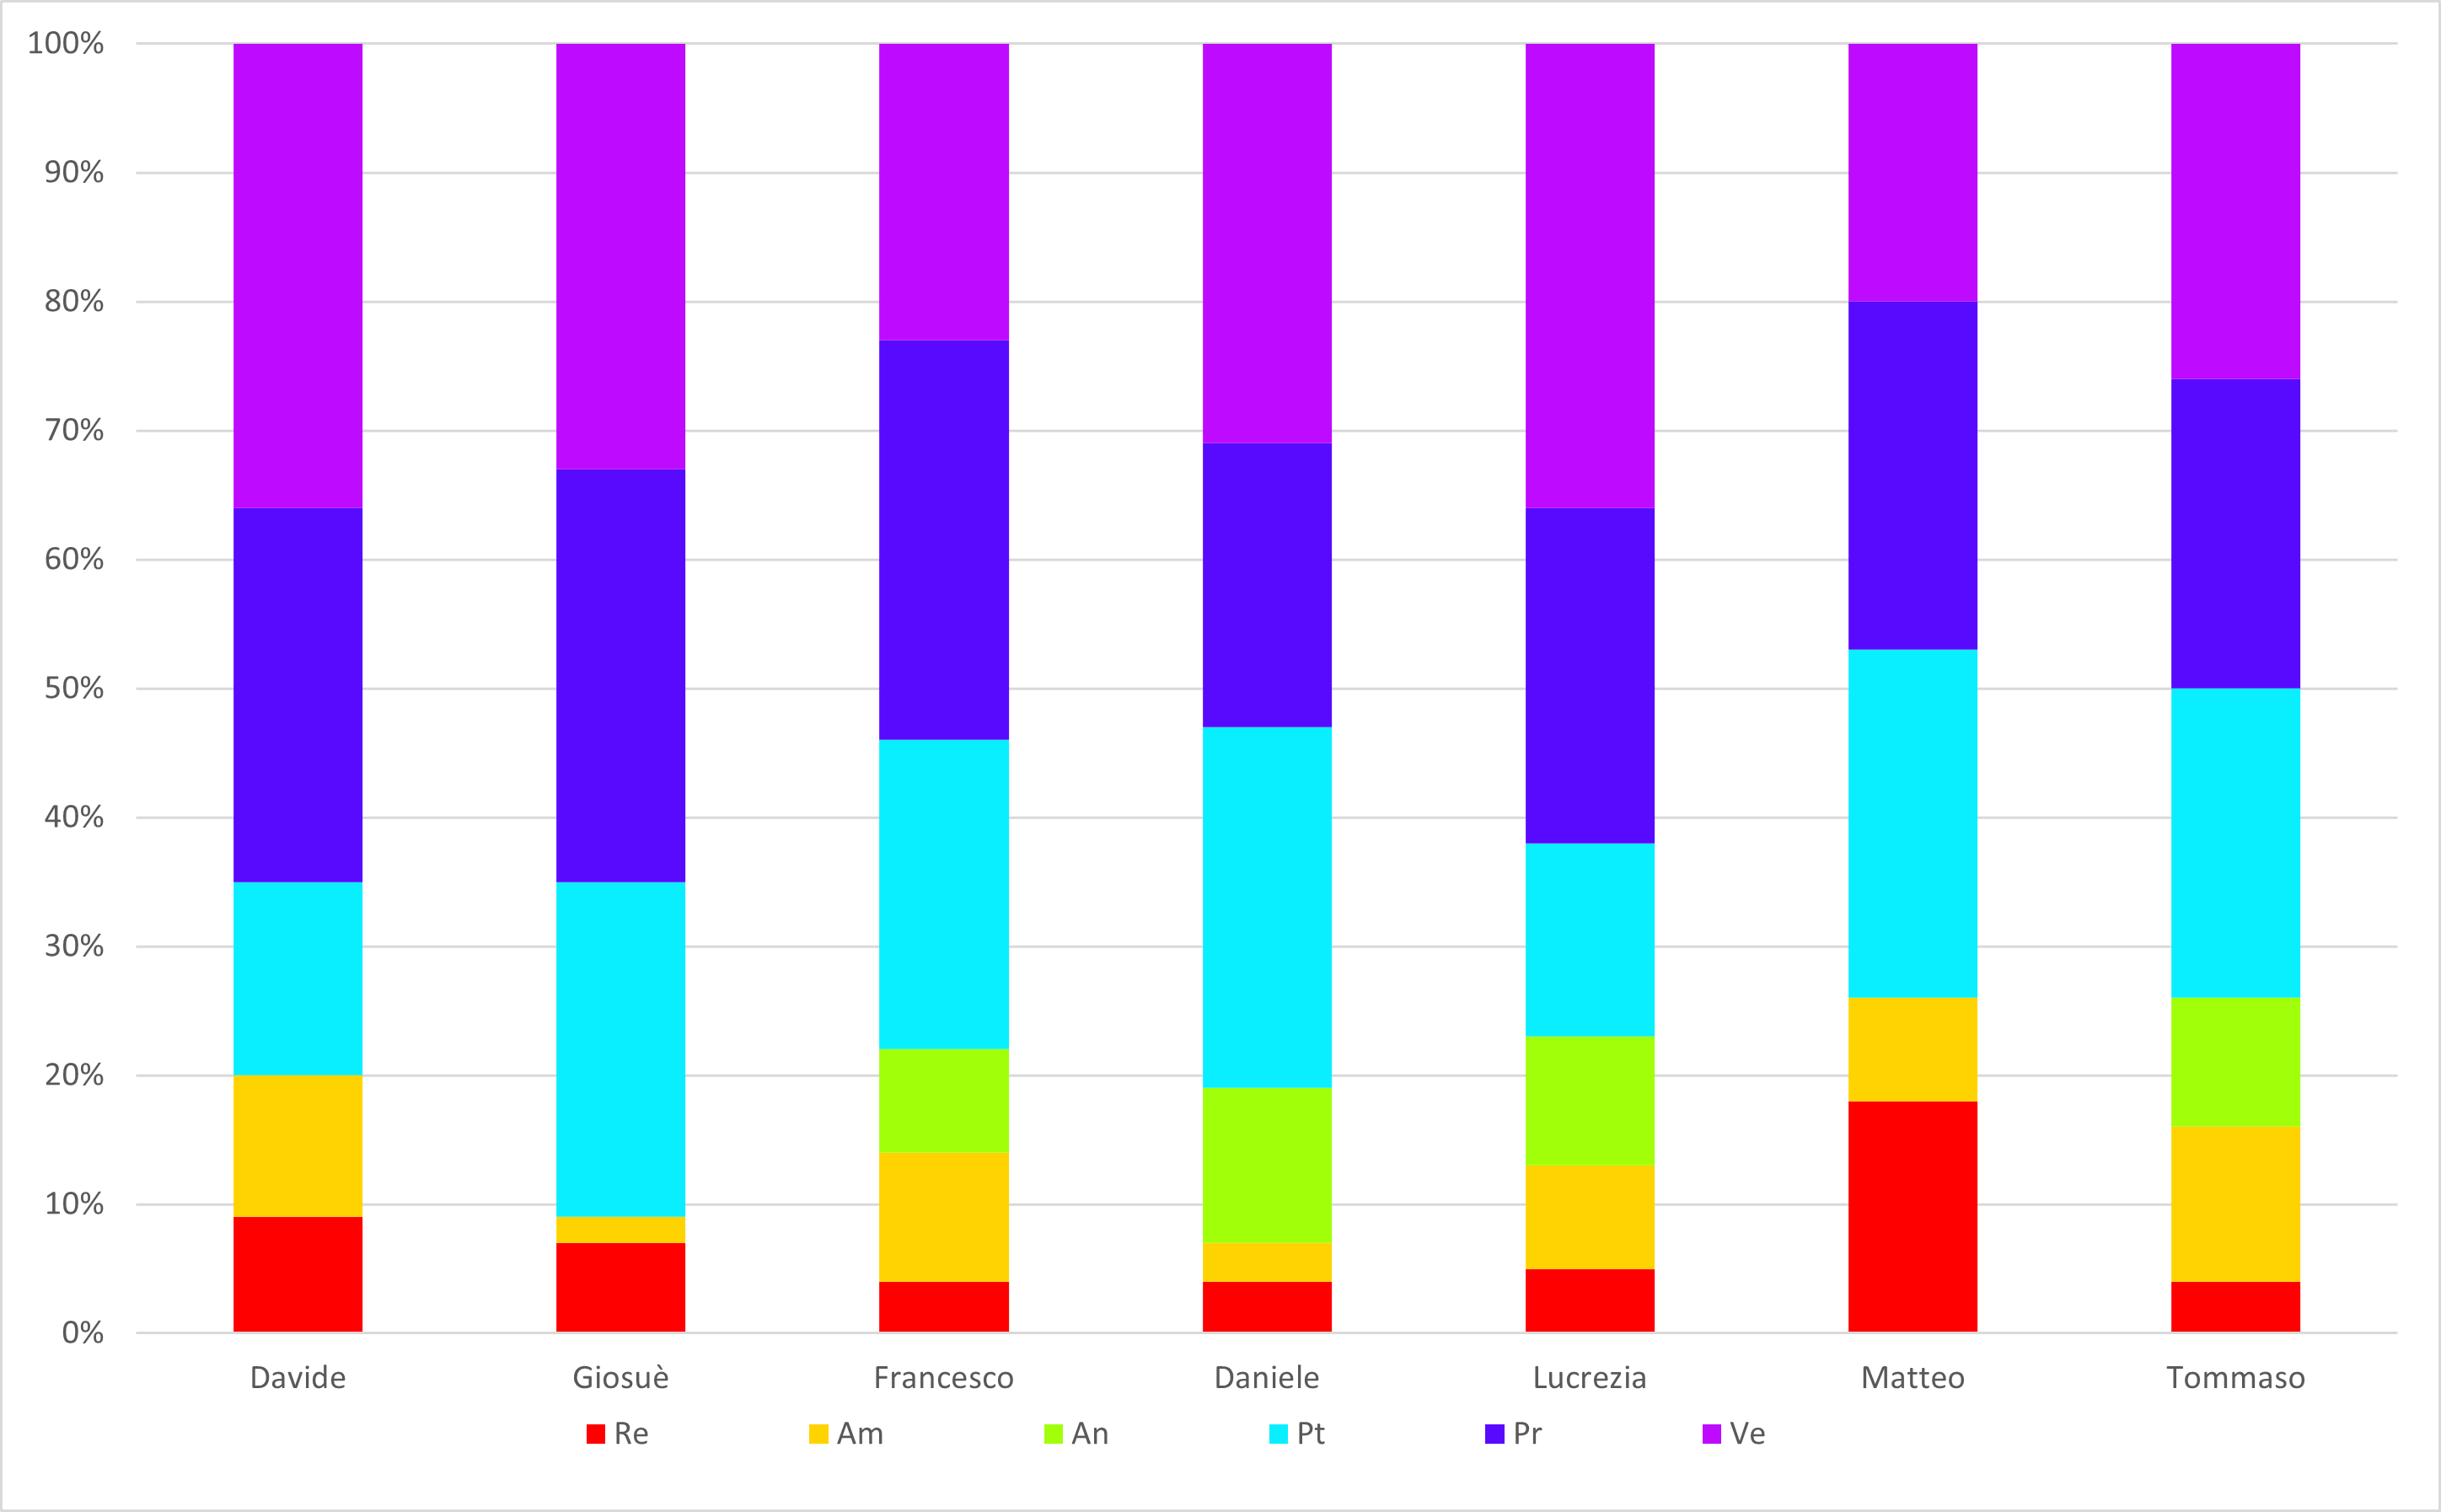
\includegraphics[scale = 0.5]{components/img/Totale-rendicontate-isto.png}
    \caption{ Istogramma della ripartizione delle ore rendicontate}
    \label{fig:Istogramma ripartizione ore totali rendicontate}
\end{figure}
\paragraph{Prospetto economico}
Il costo totale rendicontato per ogni ruolo è il seguente:
\begin{table}[H]
		\begin{center}
			\setlength{\aboverulesep}{0pt}
			\setlength{\belowrulesep}{0pt}
			\setlength{\extrarowheight}{.75ex}
			\rowcolors{2}{AzzurroGruppo!10}{white}
			\begin{tabular}{ c c c }
				\rowcolor{AzzurroGruppo!30} 
				\textbf{Ruolo} & \textbf{Ore} & \textbf{Costo} \\
				\toprule
				Responsabile   & 51 & 1530 \euro \\
				Amministratore & 54 & 1080 \euro \\
				Analista       & 40 & 1000 \euro \\
				Progettista    & 159 & 3498 \euro \\
				Programmatore  & 191 & 2865 \euro \\
				Verificatore   & 205 & 3075 \euro \\
				\textbf{Totale} & \textbf{700} & \textbf{13048 \euro} \\
				\bottomrule
			\end{tabular}
			\caption{Prospetto dei costi delle ore rendicontate}
		\end{center}
	\end{table}
I dati ottenuti si possono riassumere nel seguente areogramma:
\begin{figure}[H]
    \centering
    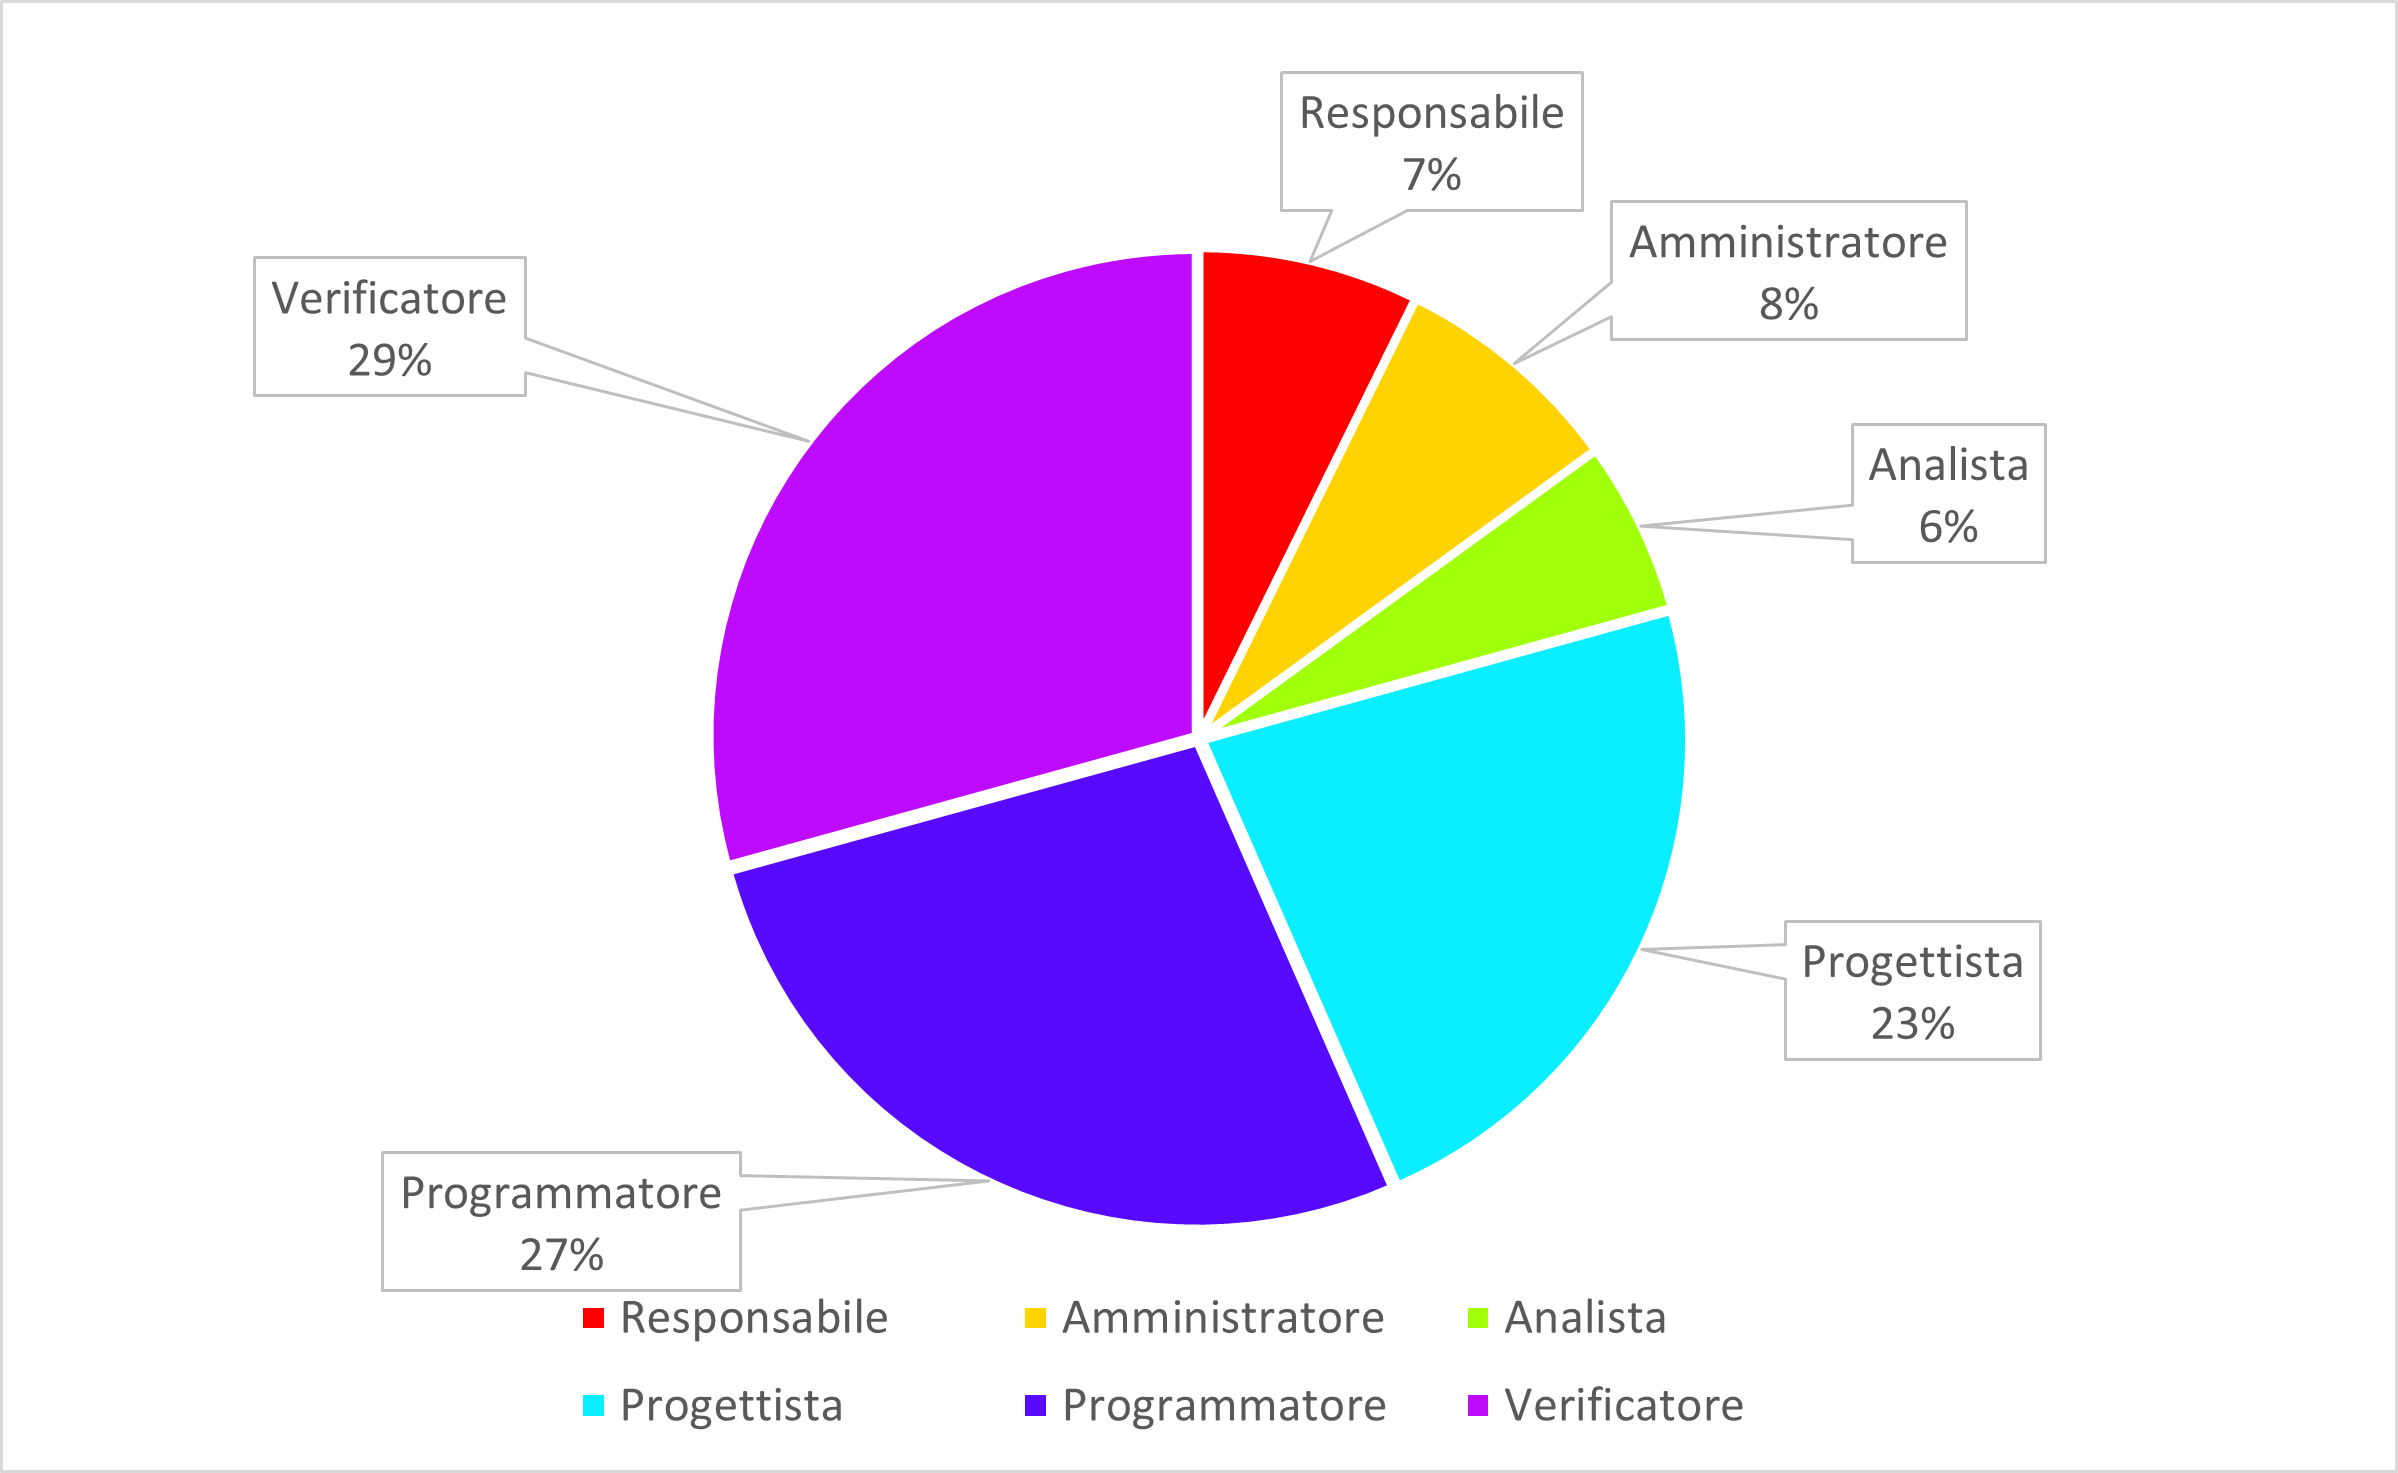
\includegraphics[scale = 0.5]{components/img/Totale-rendicontate-torta.png}
    \caption{ Areogramma delle ore rendicontate per ruolo}
    \label{fig:Areogramma ripartizione ore totali rendicontate}
\end{figure}
\subsubsection{Conclusioni}
il costo totale preventivato è : 13048 \euro .